%% (Master) Thesis template
% Template version used: v1.4
%
% Largely adapted from Adrian Nievergelt's template for the ADPS
% (lecture notes) project.


\documentclass{llncs}

%% Packages
%% ========

%% LaTeX Font encoding -- DO NOT CHANGE
\usepackage[OT1]{fontenc}

%% Babel provides support for languages.  'english' uses British
%% English hyphenation and text snippets like "Figure" and
%% "Theorem". Use the option 'ngerman' if your document is in German.
%% Use 'american' for American English.  Note that if you change this,
%% the next LaTeX run may show spurious errors.  Simply run it again.
%% If they persist, remove the .aux file and try again.
\usepackage[english]{babel}

%% Input encoding 'utf8'. In some cases you might need 'utf8x' for
%% extra symbols. Not all editors, especially on Windows, are UTF-8
%% capable, so you may want to use 'latin1' instead.
\usepackage[utf8]{inputenc}

%% The AMS-LaTeX extensions for mathematical typesetting.  Do not
%% remove.
\usepackage{amsmath,amssymb,amsfonts,mathrsfs}

%% LaTeX' own graphics handling
\usepackage{graphicx}

%% This allows you to add .pdf files. It is used to add the
%% declaration of originality.
\usepackage{pdfpages}

%% Some more packages that you may want to use.  Have a look at the
%% file, and consult the package docs for each.
%% See the TeXed file for more explanations

%% [OPT] Multi-rowed cells in tabulars
%\usepackage{multirow}

%% [REC] Intelligent cross reference package. This allows for nice
%% combined references that include the reference and a hint to where
%% to look for it.
\usepackage{varioref}

%% [OPT] Easily changeable quotes with \enquote{Text}
%\usepackage[german=swiss]{csquotes}

%% [REC] Format dates and time depending on locale
\usepackage{datetime}

%% [OPT] Provides a \cancel{} command to stroke through mathematics.
%\usepackage{cancel}

%% [NEED] This allows for additional typesetting tools in mathmode.
%% See its excellent documentation.
\usepackage{mathtools}

%% [ADV] Conditional commands
%\usepackage{ifthen}

%% [OPT] Manual large braces or other delimiters.
%\usepackage{bigdelim, bigstrut}

%% [REC] Alternate vector arrows. Use the command \vv{} to get scaled
%% vector arrows.
% \usepackage[h]{esvect}

%% [NEED] Some extensions to tabulars and array environments.
\usepackage{array}

%% [OPT] Postscript support via pstricks graphics package. Very
%% diverse applications.
%\usepackage{pstricks,pst-all}

%% [?] This seems to allow us to define some additional counters.
%\usepackage{etex}

%% [ADV] XY-Pic to typeset some matrix-style graphics
%\usepackage[all]{xy}

%% [OPT] This is needed to generate an index at the end of the
%% document.
%\usepackage{makeidx}

%% [OPT] Fancy package for source code listings.  The template text
%% needs it for some LaTeX snippets; remove/adapt the \lstset when you
%% remove the template content.
\usepackage{listings}
\lstset{language=TeX,basicstyle={\normalfont\ttfamily}}

%% [REC] Fancy character protrusion.  Must be loaded after all fonts.
\usepackage{microtype}

%% [REC] Nicer tables.  Read the excellent documentation.
\usepackage{booktabs}

%% Own packages
\usepackage{caption}
\usepackage{subcaption}
\captionsetup{subrefformat=parens}


%% Helpful macros.
%% Special characters for number sets, e.g. real or complex numbers.
\newcommand{\C}{\mathbb{C}}
\newcommand{\K}{\mathbb{K}}
\newcommand{\N}{\mathbb{N}}
\newcommand{\Q}{\mathbb{Q}}
\newcommand{\R}{\mathbb{R}}
\newcommand{\Z}{\mathbb{Z}}
\newcommand{\X}{\mathbb{X}}

%% Fixed/scaling delimiter examples (see mathtools documentation)
\DeclarePairedDelimiter\abs{\lvert}{\rvert}
\DeclarePairedDelimiter\norm{\lVert}{\rVert}
\DeclarePairedDelimiter\bracks{\lbrack}{\rbrack}
\DeclarePairedDelimiter\ceil{\lceil}{\rceil}

%% Use the alternative epsilon per default and define the old one as \oldepsilon
\let\oldepsilon\epsilon
\renewcommand{\epsilon}{\ensuremath\varepsilon}

%% Also set the alternate phi as default.
\let\oldphi\phi
\renewcommand{\phi}{\ensuremath{\varphi}}

%% Custom commands
\newcommand{\pr}[1]{\Pr\bracks*{#1}}

\ifdefined\thesisfinal
	\newcommand{\question}[1]{}
	\newcommand{\todo}[1]{}
\else
	\newcommand{\question}[1]{\textcolor{magenta}{\textbf{Q:} #1}}
	\newcommand{\todo}[1]{\textcolor{red}{\textbf{TODO:} #1}}
\fi

\newcommand{\from}{\leftarrow}
\newcommand{\gen}{\mathrm{Gen}}
\newcommand{\enc}{\mathrm{Enc}}
\newcommand{\dec}{\mathrm{Dec}}
\newcommand{\hgen}{H_\mathrm{gen}}
\newcommand{\fhgen}{\mathcal{H}_\mathrm{gen}}
\newcommand{\qgen}{Q_\mathrm{gen}}
\newcommand{\hdep}{H_\mathrm{dep}}
\newcommand{\fhdep}{\mathcal{H}_\mathrm{dep}}
\newcommand{\qdep}{Q_\mathrm{dep}}
\newcommand{\hdh}{H_\mathrm{DH}}
\newcommand{\fdh}{F_\mathrm{DH}}
\newcommand{\fhdh}{\mathcal{H}_\mathrm{DH}}
\newcommand{\qdh}{Q_\mathrm{DH}}
\newcommand{\mdh}{m_\mathrm{DH}}
\newcommand{\qs}{Q_\mathrm{s}}
\newcommand{\ms}{m_\mathrm{s}}
\newcommand{\eeav}{\epsilon_\mathrm{EAV}}
\newcommand{\eddh}{\epsilon_\mathrm{DDH}}

% adversary
\newcommand{\adv}{\mathcal{A}}
\newcommand{\wins}{\mathcal{A} \text{ wins}}

% games and advantage
\newcommand{\game}[3]{\mathrm{Game}_{#1, #2}^{\mathrm{#3}}}
\newcommand{\advantage}[3]{\mathrm{Adv}_{#1, #2}^{\mathrm{#3}}}

% schemes
\newcommand{\dhies}{\Pi_{\mathrm{DH}}}
\newcommand{\treekem}{\Sigma_{\mathrm{TK}}}

%% ===============


%% Make document internal hyperlinks wherever possible. (TOC, references)
%% This MUST be loaded after varioref, which is loaded in 'extrapackages'
%% above.  We just load it last to be safe.
\usepackage[bookmarks,bookmarksopen,bookmarksdepth=2,linkcolor=black,colorlinks=true,citecolor=black,filecolor=black]{hyperref}


%% Document information
%% ====================

\title{Tighter Security for Group Key Agreement in the Random Oracle Model}
\author{Andreas Ellison \and Karen Klein}
\institute{ETH Zurich, Switzerland \\
	\email{\{andreas.ellison,karen.klein\}@inf.ethz.ch}
}

\begin{document}

\maketitle

%% The abstract of your thesis.  Edit the file as needed.
\begin{abstract}
	The Messaging Layer Security (MLS) protocol, recently standardized in RFC 9420, aims to provide efficient asynchronous group key establishment with strong security guarantees. The main component of MLS, which is the source of its key efficiency and security properties, is a protocol called TreeKEM. Given that a major vision for the MLS protocol is for it to become the new standard for messaging applications like WhatsApp, Facebook Messenger, Signal, etc., it has the potential to be used by a huge number of users. Thus, it is important to better understand the security of MLS and hence also of TreeKEM. In work by Klein et.\ al, TreeKEM was proven adaptively secure in the Random Oracle Model (ROM) with a polynomial loss in security by proving a result about the security of an arbitrary IND-CPA secure public-key encryption scheme in a public-key version of the Generalized Selective Decryption (GSD) security game. \\


	In this work, we prove a tighter bound for the security of TreeKEM that implies meaningful security guarantees in practice. We follow the approach of Klein et.\ al and first introduce a modified version of the public-key GSD game better suited for analyzing TreeKEM. We then provide a simple and detailed proof of security for a specific encryption scheme, the DHIES scheme (currently the only standardized scheme in MLS), in this game in the ROM and achieve a smaller security loss compared to the result from Klein et.\ al. Finally, we state the result on the security of TreeKEM implied by this bound, and give an interpretation of the result with protocol parameters used in practice.

	\keywords{Messaging Layer Security \and TreeKEM \and Secure Messaging \and Group Key-Agreement \and Adaptive Security \and DHIES}
\end{abstract}


%% Your real content!
\section{Introduction}

We all rely on messaging applications like WhatsApp, Facebook Messenger, Signal, etc.\ in our daily lives and take it for granted that our messages will be transmitted securely, for some definition of ``secure''. A common security feature expected from the protocol employed in a messaging application is end-to-end encryption, i.e.\ that only the end users of a messaging session can read the messages being sent and the service provider or any party with access to the communication channel learns nothing of their contents. The protocol should work in an asynchronous setting: we would like to send messages even when the recipient is offline, and we expect them to receive the message once they come online. For this, we must rely on a delivery service to store and deliver the messages. Of course, also this delivery service should learn nothing from the messages.

There are two more advanced security features expected from messaging protocols today, both related to security in case a user is compromised:
\begin{itemize}
	\item forward secrecy (FS): the compromise should not reveal the contents of old messages
	\item post-compromise security (PCS): after the user recovers from the compromise, new messages are secure once again
\end{itemize}
As a user may well not know that they have been compromised, ensuring PCS requires regularly updating the key material used for encryption (in a way that the information leaked in a compromise \emph{before} the update does not suffice to compute encryption keys used \emph{after} the update). The more often the key material is updated, the stronger the level of PCS that is achieved. Thus, updating the key material should be an efficient operation.

For messaging between two users, the Double Ratchet protocol \cite{double-ratchet}, the main component of the Signal Protocol, is a widely adopted solution used by major messaging applications such as Signal, WhatsApp, Facebook Messenger and more. It is well-studied and achieves all of the above security guarantees \cite{double-ratchet-analysis}. For messaging in a group of more than two users, a straightforward solution is to maintain 1:1 communication channels using the Double Ratchet protocol between every pair of users and send messages to the group by sending them to every member individually. This achieves very strong security guarantees but requires a number of encryption operations linear in the group size to send a message.

Another common solution is to use sender keys \cite{sender-keys}: every user creates a symmetric key, their \emph{sender key}, and distributes this sender key to every other user using 1:1 channels as before. A user sending a message then derives a symmetric encryption key for the message from their sender key, while continually updating their sender key (with each sent message) to provide FS. However, achieving PCS is costly: if a user is compromised, the sender keys of all users are leaked and recovering from the compromise requires each user to send a new sender key to every other user over the respective 1:1 channels, resulting in a number of operations linear in the group size per user and a quadratic number of operations in total. Moreover, dynamic group membership introduces additional complexity:
\begin{itemize}
	\item adding a new member involves the new member sharing their sender key with all other group members
	\item removing a member requires distributing new sender keys in the group, just like recovering from a compromise
\end{itemize}
The Messaging Layer Security (MLS) protocol, recently standardized in \cite{rfc9420}, proposes a solution for group messaging with better efficiency and the same strong security guarantees as for the two-party case. Updating key material and adding or removing members can be achieved with a logarithmic number of operations (although the complexity may still degrade to linear in certain scenarios). At the core of MLS is a fairly recent primitive called a \emph{continuous group key agreement} (CGKA) scheme \cite{rtreekem} (this primitive was introduced only \emph{after} the first draft of the MLS protocol). In essence, a CGKA scheme enables a group of users to agree on a \emph{group key}, which they can then use to derive symmetric message encryption keys. This key must be indistinguishable from a random key for anyone outside the group eavesdropping on all communication. However, a CGKA scheme must also achieve FS and PCS, and support dynamic group membership. Hence, it must provide mechanisms for members to update their key material, add new users to the group and remove members from the group. Moreover, the scheme must work in the asynchronous setting with an untrusted service to deliver protocol messages.

The CGKA scheme used in the MLS protocol is called TreeKEM (initially proposed in \cite{treekem}) and the majority of the literature on MLS is dedicated to analyzing TreeKEM or proposing better CGKA schemes. We refer the reader to \cite[Section 1.3]{guillermo-thesis} for an in-depth overview of the literature. The TreeKEM protocol has undergone multiple changes since its inception. In this work, we refer to the version documented in RFC 9420. Given that the vision for the MLS protocol is for it to become the new standard for messaging protocols and that it has support from several large companies \cite{google-mls,mls-support}, it has the potential to be used by a huge number of users. Thus, understanding the security of MLS and hence also of TreeKEM is of great importance. This means having formal security guarantees about the security provided by TreeKEM (based on appropriate hardness assumptions).

\subsection{The TreeKEM protocol} \label{sec:treekem-overview}

\paragraph{Propose and commit syntax}

As a CGKA scheme, TreeKEM must support operations for updating the key material of a group member, adding a new user and removing a member. The syntax for these operations has changed over time. In the current version of MLS, the protocol uses so-called \emph{proposals} and \emph{commits}. Whenever a user would like to have their key material updated, add a new user or remove a group member, they create a corresponding \emph{update}, \emph{add} or \emph{remove proposal}, respectively, and share this proposal with the group. Any group member can then create a \emph{commit} to apply a set of proposals, create a new group key and update their key material in the process. The commit object includes (encrypted) information such that every group member can update their view of the group and compute the new group key.

\paragraph{TreeKEM dynamics}

TreeKEM uses a full binary tree to model the group and every user is associated with a leaf in the tree (the remaining leaves may be left empty). Each user maintains a synchronized view of the tree, though different users will know more about different parts of the tree. The group key is derived from the root of the tree. Every node $n$ in the tree has an associated key pair $(pk_n, sk_n)$ output by $\Pi.\gen$ where $\Pi$ is a public-key encryption scheme. All public keys are known to all users. Let the \emph{direct path} of a leaf be the path from the leaf's parent to the root. A leaf's \emph{path to the root} refers to the same path but including the leaf as well. Every user at a leaf knows the secret key of their leaf and, in the usual case, the secret keys of all nodes on their direct path, though there can be exceptions to this rule. To illustrate the scheme and how commit operations are performed, we will consider a group with users $A, B, \ldots, G$ and $H$, as depicted in Figure~\ref{fig:treekem-tree}. In the following, we will use these labels for the users both to refer to the users themselves and to their nodes in the tree.

\begin{figure}
	\begin{center}
		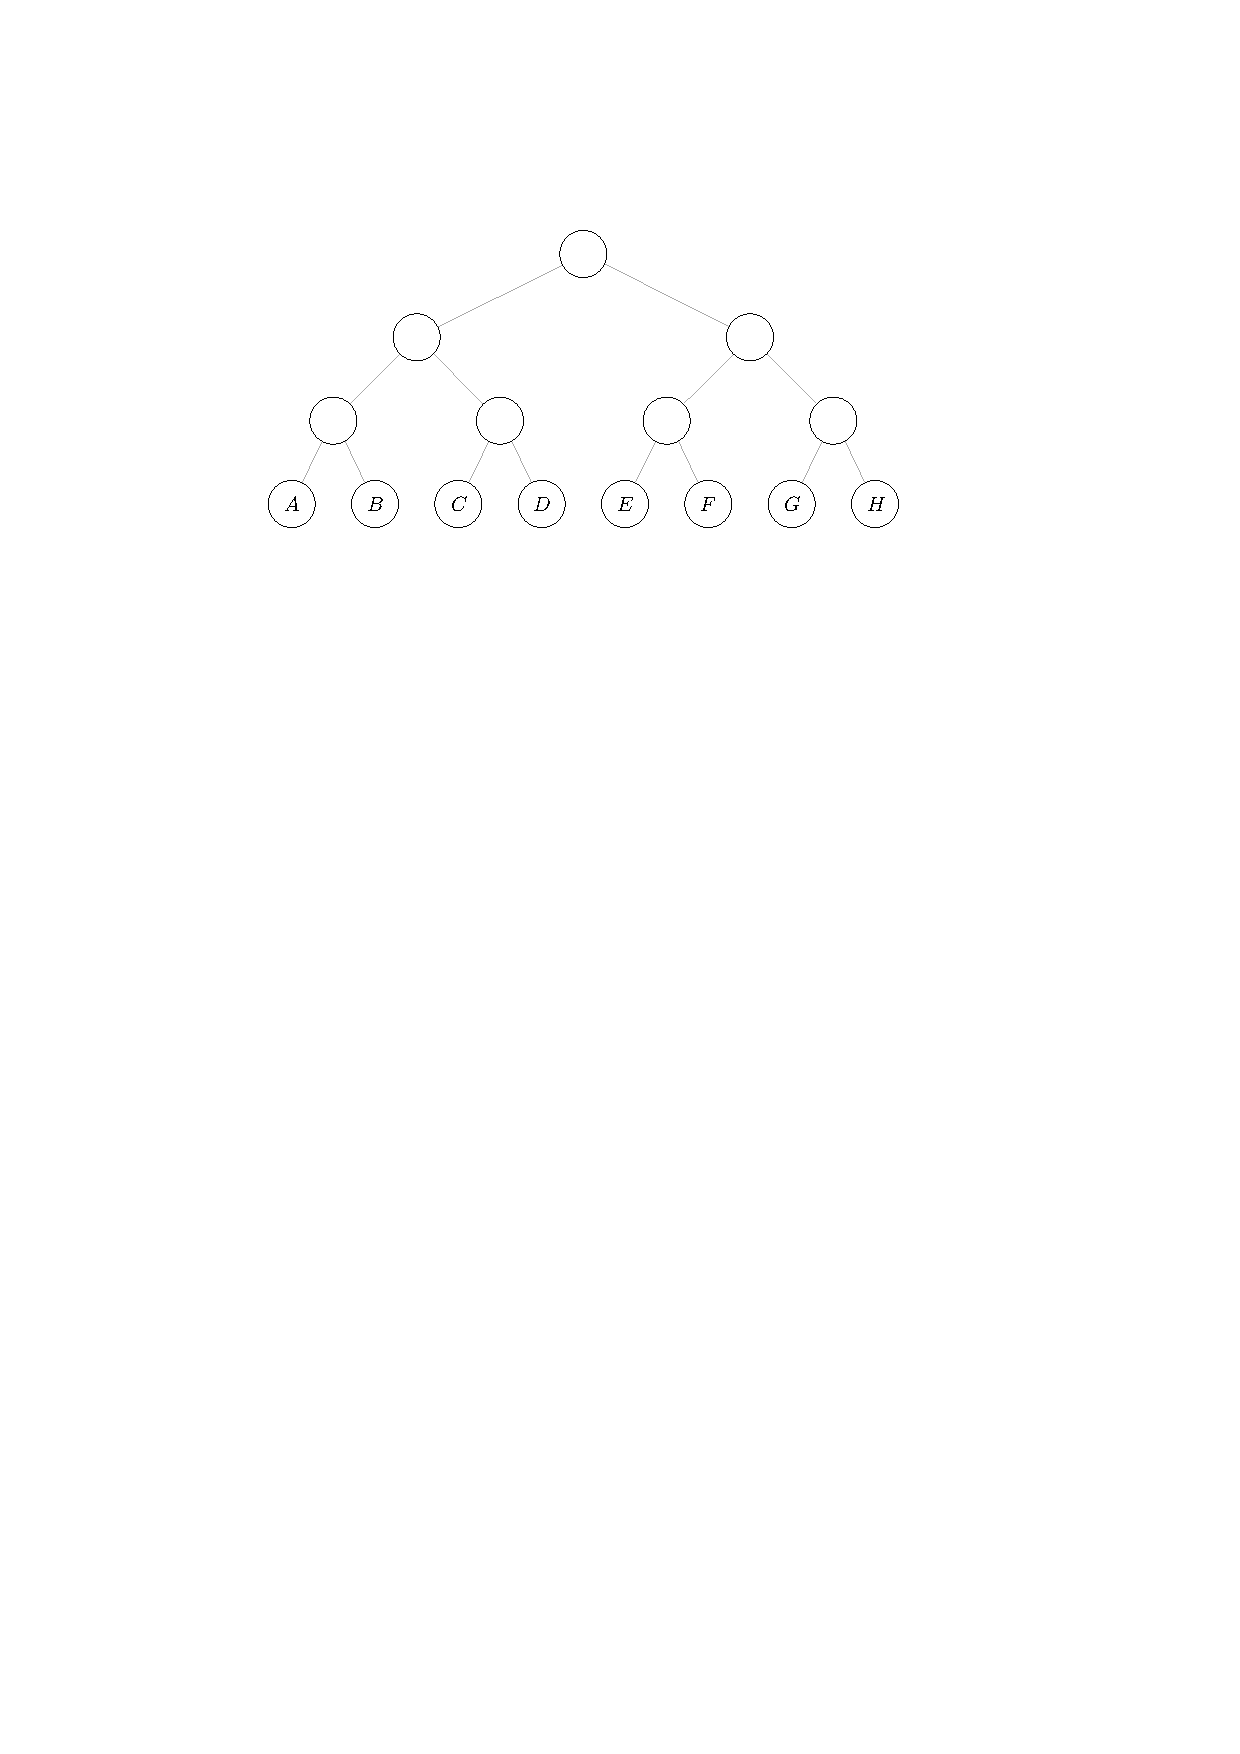
\includegraphics{figures/treekem-tree}
	\end{center}
	\caption{Illustration of a group with users 8 users in the TreeKEM protocol.}\label{fig:treekem-tree}
\end{figure}

\paragraph{Simple commits} \label{sec:simple-commit} The idea behind this tree structure is that it allows for a user creating a commit with a new group key to share the new group key with the group using only a few encryptions, while still updating all the secrets the user knew in the tree in order to recover from a possible compromise (recall that in a CGKA scheme a commit also updates the committer's key material).
To illustrate how a commit is performed and how the new group key is computed, say user $A$ performs a commit. Let us consider commits without any proposals. TreeKEM specifies two hash functions $\hgen, \hdep \colon \{0, 1\}^{\rho(\eta)} \to \{0, 1\}^{\rho(\eta)}$ where $\rho(\eta)$ gives the number of random bits used by $\Pi.\gen(1^\eta)$. The depth of user $A$ is $d = 3$. $A$ will replace all the $d + 1$ nodes on their path to the root with new nodes $A, p_1, \ldots, p_d$. (In practice $A$ would just replace the information stored in the original nodes.)
The key pairs for the new nodes are sampled as follows. For the leaf node $A$, user $A$ simply samples a key pair by running $\Pi.\gen(1^\eta)$. For the remaining nodes, they first sample $s_1 \from \{0, 1\}^{\rho(\eta)}$ and compute the key pair of the first parent $p_1$ as $\Pi.\gen(1^\eta, \hgen(s_1))$. For $i \in \{2, \ldots, d\}$ they then compute $s_i \coloneqq \hdep(s_{i - 1})$ and set the key pair of $p_i$ to be $\Pi.\gen(1^\eta, \hgen(s_i))$. The new group key is $k \coloneqq \hdep(s_{d})$.

User $A$ only needs to share (encryptions of) the seeds $s_i$ for the other users to update their view of the tree and compute the new group key:
\begin{itemize}
	\item To share the group key with user $B$, $A$ computes the ciphertext $c_1 \from \Pi.\enc_{pk_B}(s_1)$. $B$ can then compute the seed $s_1$, then use that to compute the seeds $s_2, \ldots, s_d$, the key pairs of all new nodes on their path to the root and the group key $k$.
	\item To share the new group key with users $C$ and $D$, $A$ computes the ciphertext $c_2 \from \Pi.\enc_{pk_X}(s_2)$, where $X$ is the parent of the nodes $C$ and $D$. Both $C$ and $D$ know the secret key $sk_X$ of their parent and can decrypt $c_2$.
	\item To share the new group key with users $E, F, G$ and $H$, $A$ computes the ciphertext $c_3 \from \Pi.\enc_{pk_Y}(s_3)$, where $Y$ is the right child of the root node. Again, all users under $Y$ know $sk_Y$ and can thus decrypt $c_3$.
\end{itemize}
The commit $c$ that $A$ shares with all users includes the ciphertexts $c_1, c_2$ and $c_3$ and the public keys of all new nodes. Figure~\ref{fig:treekem-simple-update} illustrates the commit performed by $A$.

\begin{figure}
	\begin{center}
		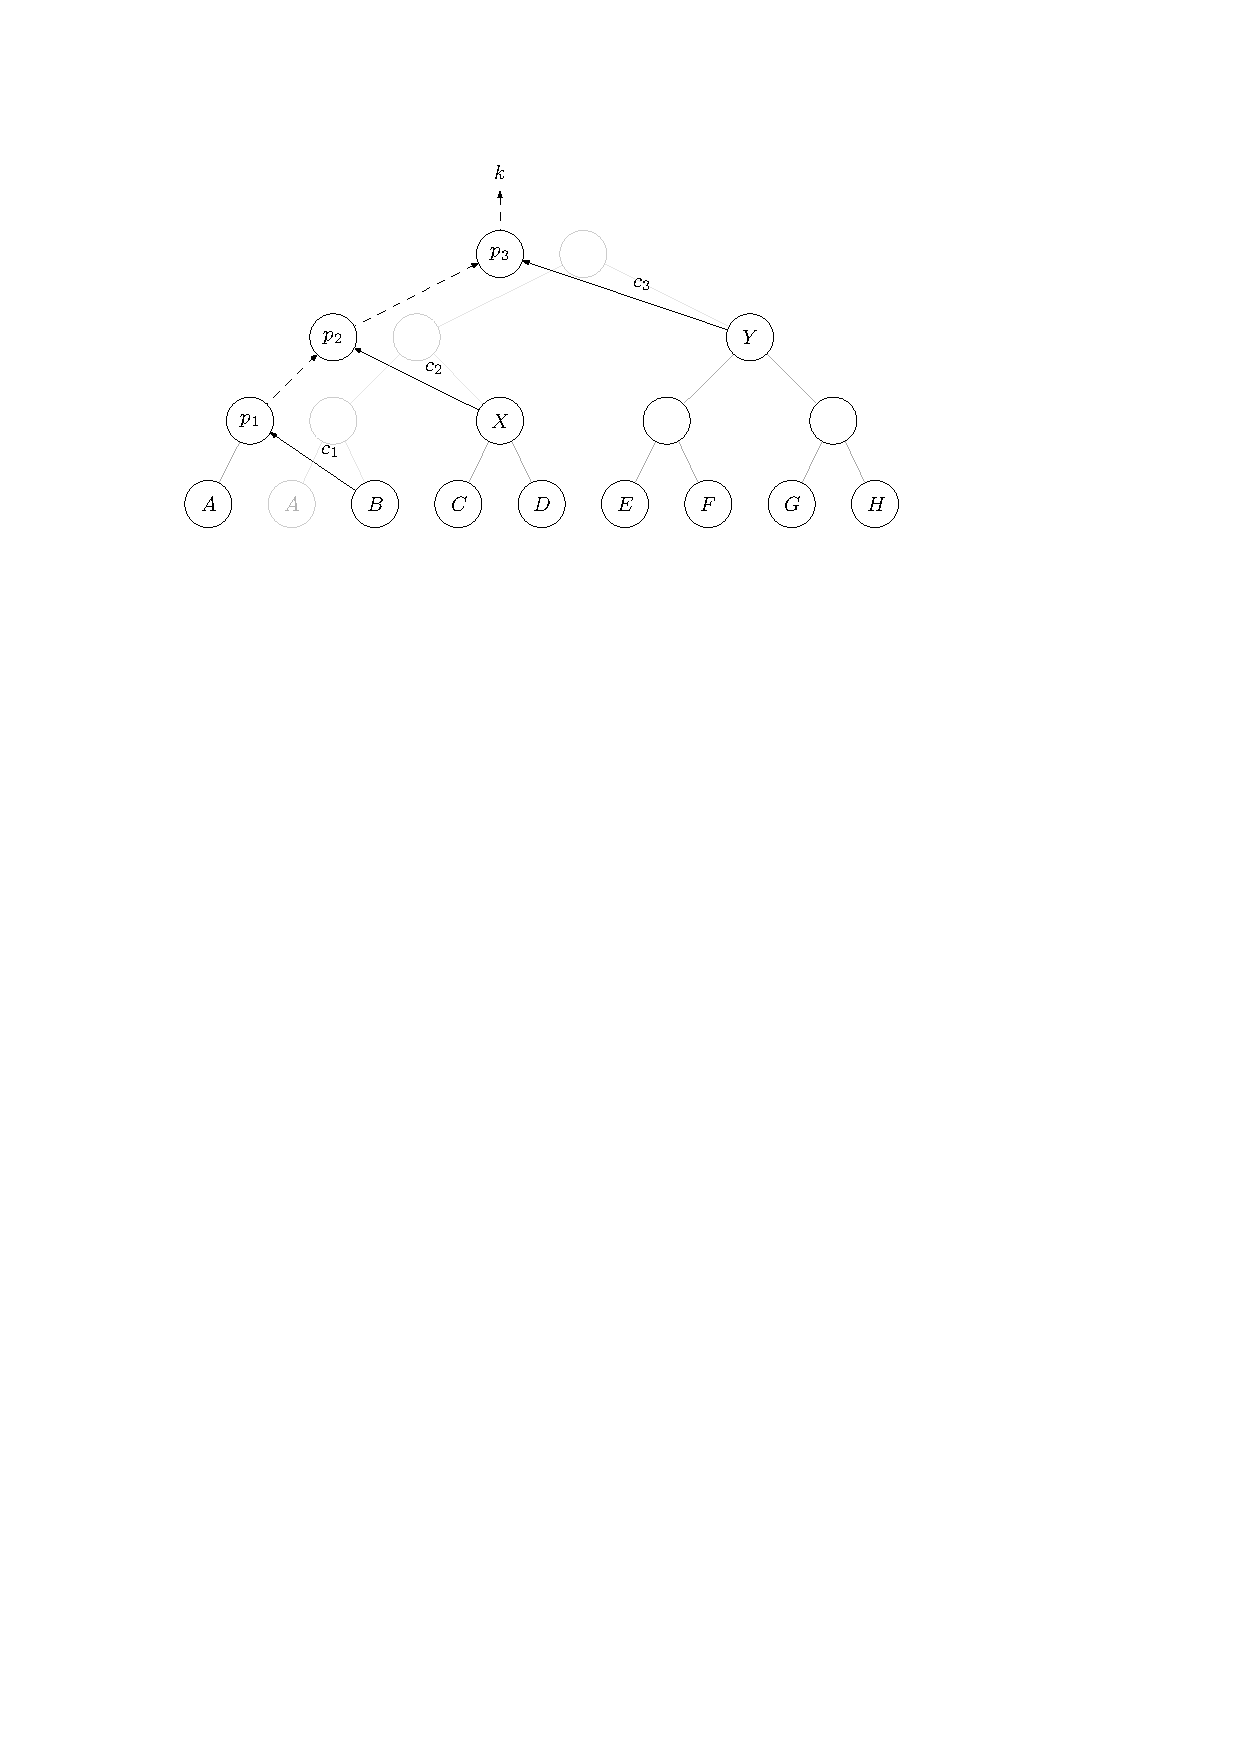
\includegraphics{figures/treekem-simple-update}
	\end{center}
	\caption{The commit by user $A$ described in the text. Dashed directed edges illustrate the fact that the target is related to the source via the hash function $\hdep$. The solid directed edges illustrate the fact that the seed of the target node is encrypted to the public key of the source node.}\label{fig:treekem-simple-update}
\end{figure}

The nodes $B, X$ and $Y$ form the \emph{copath} of $A$: the copath of a node $v$ consists of the sibling of each node on $v$'s path to the root, excluding the root itself. In the ideal case as above, a node performing a commit only has to compute one encryption for each node on its copath, i.e. logarithmically many encryptions in the total number of users.


The above concepts suffice to understand our main results. For a discussion of how proposals are incorporated into a commit, we refer the reader to Section~\ref{sec:treekem-overview-proposals} of the appendix.

\subsection{The GSD game} \label{sec:gsd-intro}

The Generalized Selective Decryption (GSD) security game \cite{gsd} was introduced precisely to analyze adaptive security for protocols based on a graph-like structure, as is the case with TreeKEM. It was initially defined for the private-key setting and later adapted to the public-key setting in \cite{ttkem}.

In the GSD security game, given an encryption scheme a graph, the \emph{GSD graph}, is constructed by the challenger where every node in the graph is associated with a symmetric key in the private-key setting, or a public/private key pair in the public-key setting. The adversary can then request encryptions of a node's (secret) key under the (public) key of another node. In the public-key setting, such an \emph{encryption query} also reveals the latter node's public key. This creates an \emph{encryption edge} in the graph, directed from the node whose (public) key was used for encryption to the node whose key was encrypted. The adversary can also corrupt any node, which reveals its (secret) key and allows the adversary to compute the (secret) key of any other node reachable from the corrupted node in the graph by performing decryptions along the path to the other node. At the end of the game the adversary chooses a node to be challenged on, the \emph{challenge node}. A coin is then tossed and the adversary is given either the (secret) key of the challenge node or a uniformly random (secret) key and it must guess which scenario it is in. The possible choices for the challenge node must of course be restricted to nodes whose keys were not compromised through a corruption, meaning that the challenge node should never be reachable from a corrupted node in the graph. Further restrictions are also necessary which we do not go into here and refer the reader to Section~\ref{sec:sd-gsd-game}. Figure~\ref{fig:gsd-example} illustrates what an example GSD graph may look like.

\begin{figure}
	\begin{center}
		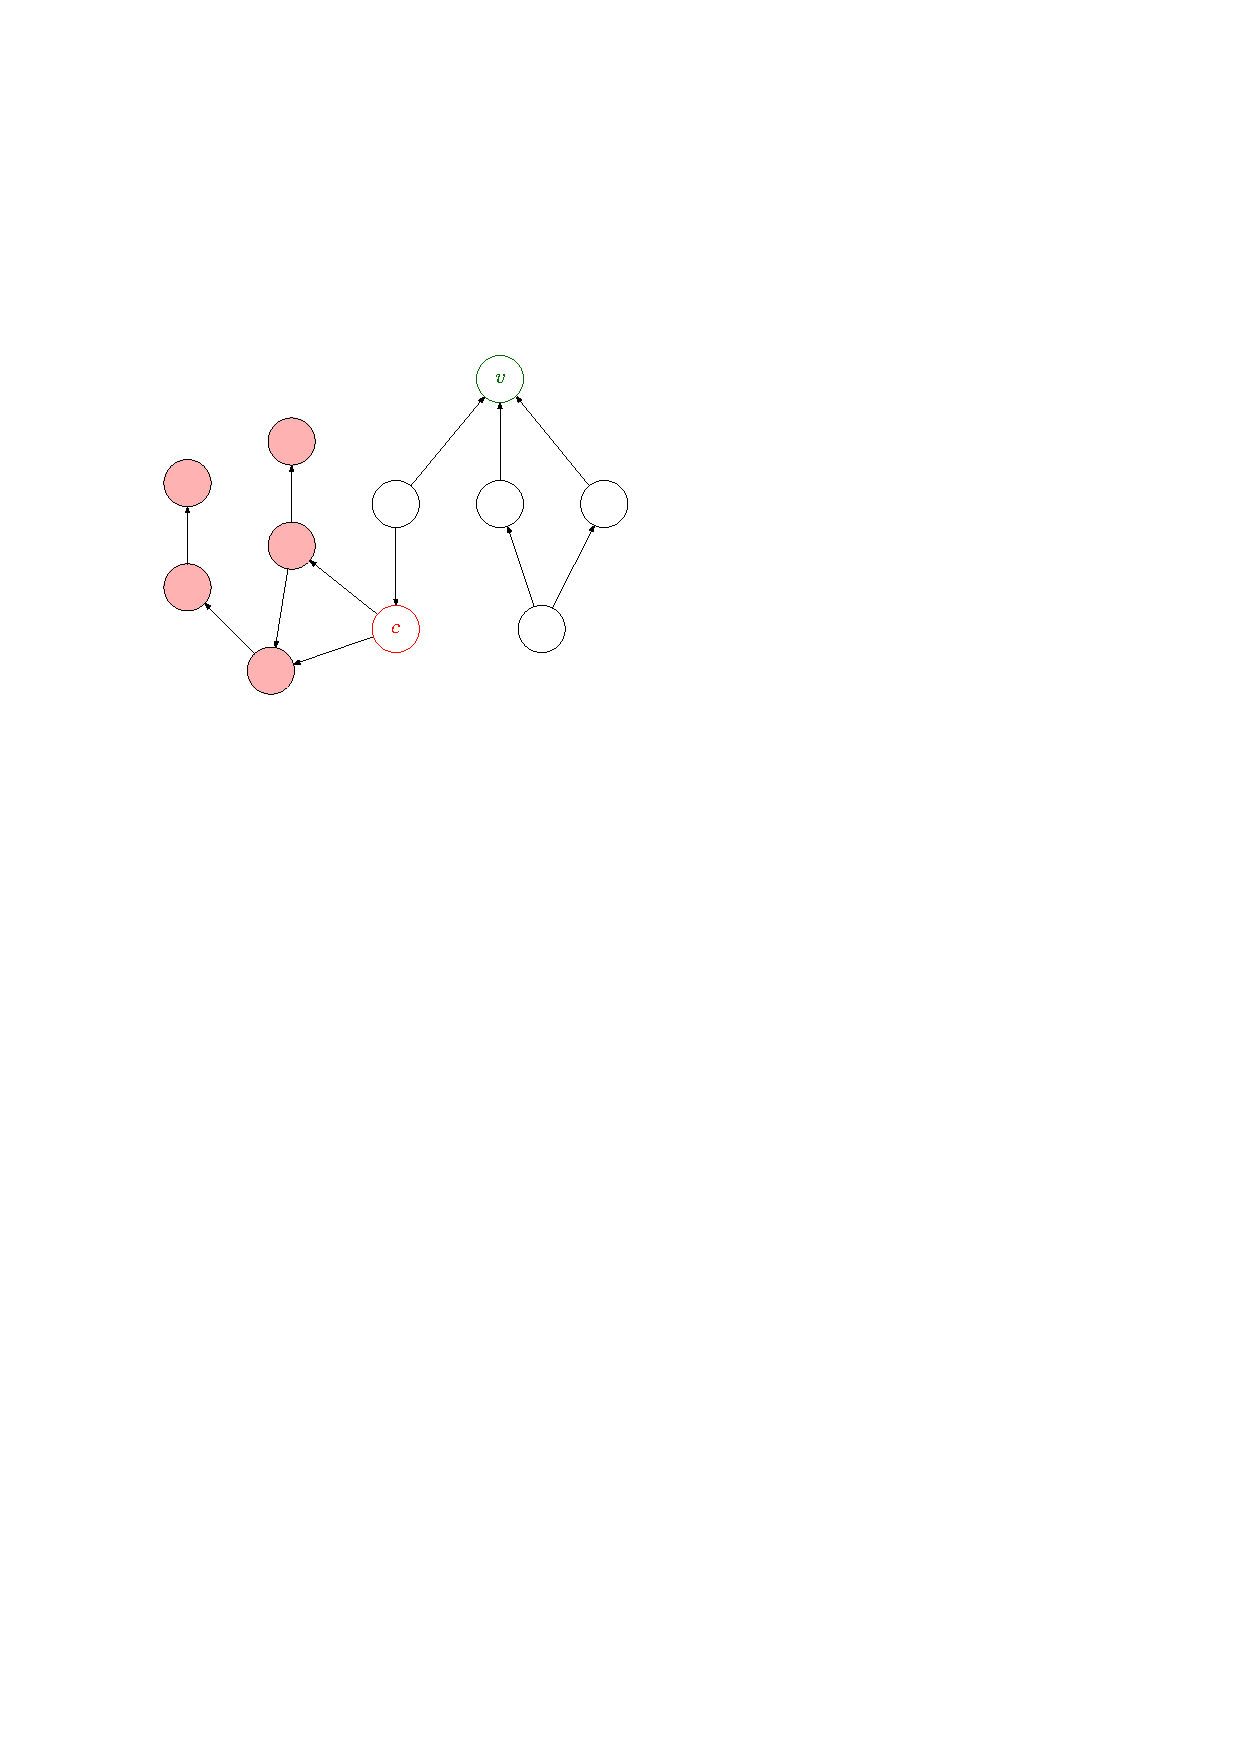
\includegraphics{figures/gsd-example}
	\end{center}
	\caption{An illustration of the GSD graph for an instance of the GSD game. The challenge node is $v$. The node $c$ was corrupted, resulting in all nodes reachable from it being compromised, as marked with red color.} \label{fig:gsd-example}
\end{figure}

The graph constructed in the public-key GSD game and the tree structure behind the TreeKEM protocol clearly resemble each other. Let $\Pi$ the public-key encryption scheme in use, where $\Pi.\gen(1^\eta)$ samples $\rho(\eta)$ random bits. We can make some small modifications to the public-key GSD game such that the operations performed in TreeKEM match the ones performed in this modified GSD game. Take the functions $\hgen, \hdep$ used in TreeKEM and first modify the game as follows:
\begin{itemize}
	\item the key pair of a node $v$ is generated by sampling a seed $s_v \in \{0, 1\}^{\rho(\eta)}$ and computing $(pk_v, sk_v) = \Pi.\gen(1^\eta, \hgen(s_v))$
	\item encryption queries encrypt the seed of the target node instead of its secret key
\end{itemize}
Now the generation of key pairs and the encryptions computed in TreeKEM match what is done in this adapted GSD game. To model the fact that in TreeKEM the seed of a node may depend on the seed of another node through $\hdep$ (as in the new direct path computed in a commit), we can introduce a new type of edge which we call a \emph{seed dependency}: a seed dependency $(u, v)$ implies that $s_v = \hdep(s_u)$.

\subsection{Existing security proofs}

The work in \cite{ttkem} made use of the relationship between the (public-key) GSD game and TreeKEM described in the previous section. They proved a polynomial bound for the adaptive security of the public-key GSD game in the Random Oracle Model (ROM) \cite{rom} for an arbitrary IND-CPA secure public-key encryption scheme. The core idea behind their proof is simple. Intuitively, the only way for an adversary to learn about the seed of an uncorrupted node for the first time is through the encryption edges into the node. The authors show that in the ROM, one can reduce security in the GSD game to the IND-CPA security of the public-key encryption scheme with a moderate security loss. They apply standard guessing arguments and a clever, albeit complicated, hybrid argument to achieve a security loss in $\mathcal{O}(N^2)$, where $N$ is the number of nodes in the GSD graph. The $N^2$ loss stems from the fact that two nodes in the GSD graph need to be guessed correctly for the reduction to succeed.

This result implies a polynomial bound for the security of TreeKEM as a CGKA scheme as outlined in \cite[Theorem 4]{ttkem} and subsequently proven in more detail in \cite[Theorem 12]{modular-group-messaging}, and was the first proof of adaptive security for TreeKEM. As far as we know, this is the tightest result on the security of TreeKEM in the literature.

\subsection{Security model}

We prove adaptive CGKA security of TreeKEM for a single group and a single challenge query when the DHIES scheme is used. Additionally, our result easily extends to adversaries performing multiple challenge queries with the same security loss (irrespective of the number of challenges). Our security definition is very close to the definition provided in \cite[Section 4.1.2]{modular-group-messaging}, but gives the adversary less power. We provide a weaker definition in order to simplify the definition and proof. However, we are confident that the exact same result can be proven for the CGKA security definition in \cite{modular-group-messaging}. The additional power given to the adversary in \cite{modular-group-messaging} should only affect the set of commits that the adversary can ask to be challenged on in the CGKA security game (defined in Section~\ref{sec:cgka} of the appendix).

\subsection{Contributions}

\paragraph{Tighter GSD security for DHIES} In this work, we formally prove the adaptive security of a specific public-key encryption scheme, the DHIES  scheme \cite{dhies}, in the adapted public-key GSD game described above, in the ROM. Focusing on the DHIES scheme allows us to achieve a tighter bound than the one in \cite{ttkem}. Each encryption of a seed $s_v$ with DHIES is a tuple of the form $\langle g^{x}, c \rangle$ with $c \from \Pi_s.\enc_{k}(s_v)$, where $k = \hdh(g^{x y})$, $g$ is a generator in the Diffie-Hellman group, $\Pi_s$ is the private-key encryption scheme used in DHIES, $\hdh$ is a hash function and $y$ is the secret key of the source node of the encryption edge. By modelling $\hdh$ as a random oracle, we know that in order for an adversary to learn anything from this encryption, intuitively, they must have either learned $k$ by querying $\hdh$ and then decrypting the ciphertext $c$, or they must have gleaned information from $c$ without knowing the key $k$. We can reduce the first case to the hardness of the Diffie-Hellman problem with a security loss in $\mathcal{O}(N)$. To achieve a linear loss, we first guess the node $v$ for which the Diffie-Hellman problem was solved on an outgoing encryption edge and exploit the self-reducibility property of the Diffie-Hellman problem in order to embed a single Diffie-Hellman challenge into all outgoing edges. The second case can be reduced to the security of the private-key encryption scheme with a security loss in $\mathcal{O}(\delta \cdot N)$ where $\delta$ is the maximum in-degree in the GSD graph.
This follows from guessing the target node $s_v$ and then applying a standard hybrid argument to the up to $\delta$ encryption edges ending in $v$.\footnote{The same hybrid argument does not work for directly reducing to the security of the public-key encryption scheme due to a technicality.} In Section~\ref{sec:tighter-mis-eav-security} of the appendix we show that the security loss can be reduced to $\mathcal{O}(N)$ for a very specific set of schemes.

Besides providing a tighter bound, our proof has further significant advantages. Arguably, it is more intuitive and less complex than the ones in \cite{modular-group-messaging,ttkem}. Furthermore, our approach can easily be adapted to prove the same security loss in a GSD game with multiple challenge queries. Both of these advantages stem from how we compute the challenge in our GSD definition. See Section~\ref{sec:sd-gsd-game} for details.

\paragraph{The security of TreeKEM} Our final result for TreeKEM has a security loss in $\mathcal{O}(u \cdot (c \cdot \log(u) + p))$ reducing to EAV security\footnote{EAV security is implied by IND-CPA security. See Section~\ref{sec:security-definitions} of the appendix for details.} of the private-key encryption scheme  and a loss in $\mathcal{O}(c \cdot \log(u) + p)$ reducing to the hardness of the Diffie-Hellman problem, where $c$ is the number of commits, $p$ the number of add or update proposals and $u$ the number of users. As with GSD, our result holds irrespective of the number of challenge queries. The result in \cite{ttkem} implies a security loss of $\mathcal{O}((c \cdot \log(u) + p)^2)$ for a single challenge query, reducing to IND-CPA security of the public-key encryption scheme. It seems clear that generalizing the proof to multiple challenges would yield a hybrid loss.
When $p$ is small such that $p \le c \cdot \log(u)$, the losses simplify to $\mathcal{O}(c \cdot u \cdot \log(u))$ and $\mathcal{O}(c \cdot \log(u))$, respectively, as opposed to $\mathcal{O}((c \cdot \log(u))^2)$ in \cite{ttkem}. In this setting, our result guarantees 90 bits of security with 128-bit parameters and 210 bits with 256-bit parameters for large groups (under standard assumptions).
When $p$ is large, e.g. when many updates are applied in each commit, the losses simplify to $\mathcal{O}(c \cdot u^2)$ and $\mathcal{O}(c \cdot u)$ as opposed to $\mathcal{O}((c \cdot u)^2)$ in \cite{ttkem}. Our result guarantees 95 bits of security when a 128-bit Diffie-Hellman group is combined with 256-bit AES, while the result in \cite{ttkem} only guarantees 64 bits. Using 256-bit parameters gives a 209-bit security level.

\subsection{Relation to MLS security}
The work in \cite{modular-group-messaging} provides a comprehensive security definition for group messaging protocols and reduces the security of MLS to the security of its underlying primitives, including the CGKA scheme. Since our proof can be adapted to work with the CGKA definition used in this work, our result implies a tighter result for the security of MLS as a whole. However, the security proof of MLS in \cite{modular-group-messaging} has a very large (but polynomial) loss and even with our improved bound for TreeKEM we don't expect this to provide a meaningful level of security. Therefore, finding a tighter reduction for the MLS protocol as a whole is a crucial open problem on the path to proving meaningful security guarantees for the protocol.


\section{Preliminaries}

Our definitions were adapted from \cite{introduction-to-modern-cryptography}. A summary of our notation, some simple lemmas, definitions for private-key and public-key encryption, IND-CPA security, EAV security, group-generation algorithms and the Decisional Diffie-Hellman (DDH) problem, and an explanation of the Random Oracle Model (ROM) can be found in \cite[Section~\ref*{sec:preliminaries-appendix}]{full-version}.

\subsection{DHIES}

In the following definition we will refer to ``key-derivation functions''. This is only meant as a hint to the reader. We do not provide a definition here, as we will always model such a function as a random oracle.

\begin{definition}[DHIES {\cite[Construction 12.19]{introduction-to-modern-cryptography}}]
	Let $\mathcal{G}$ a group-generation algorithm (for Diffie-Hellman groups). Let $\Pi_s$ a private-key encryption scheme where $\Pi_s.\gen(1^\eta)$ samples a key u.a.r.\ from $\{0, 1\}^\eta$. Let $\fhdh = \{\hdh^{(\eta)} \mid \eta \in \N \}$ a family of key-derivation functions where $\hdh^{(\eta)} \colon \{0, 1\}^* \to \{0, 1\}^{\eta}$. We write $\hdh \coloneqq \hdh^{(\eta)}$ when $\eta$ is clear from the context. Define the algorithms $\gen, \enc$ and $\dec$ as follows:
	\begin{itemize}
		\item $\gen$: on input $1^\eta$ run $\mathcal{G}(1^\eta)$ to obtain $(\mathbb{G}, q, g)$. Sample $x \from [q]$ and set $h_1 \coloneqq g^x$. Set $pk \coloneqq \langle \mathbb{G}, q, g, h_1 \rangle$ and $sk \coloneqq \langle \mathbb{G}, q, g, x \rangle$, and output $(pk, sk)$.

		      The message space is the message space of $\Pi_s$.
		\item $\enc$: on input a public key $\langle \mathbb{G}, q, g, h_1 \rangle$ and a message $m$, sample $y \from [q]$, set $h_2 \coloneqq g^y, k \coloneqq \hdh(h_1^y)$,\footnote{Where for $h \in \mathbb{G}$, $\hdh(h)$ denotes the output of $\hdh$ with the binary representation of $h$ given as input.} compute $c' \from \Pi_s.\enc_k(m)$ and output the ciphertext $\langle h_2, c' \rangle$.
		\item $\dec$: on input a private key $\langle \mathbb{G}, q, g, x\rangle$ and a ciphertext $\langle h_2, c' \rangle$, compute $k \coloneqq H(h_2^x)$ and output $\Pi_s.\dec_k(c')$. If the ciphertext is not of the right form or $\Pi_s.\dec$ outputs $\bot$, output $\bot$.
	\end{itemize}
	The public-key encryption scheme $\dhies \coloneqq (\gen, \enc, \dec)$ is called the Diffie-Hellman Integrated Encryption Scheme (DHIES).

	When using the DHIES scheme later on, we will set $pk \coloneqq h $ and $sk \coloneqq x$ in $\gen$ for simplicity. In practice $\mathbb{G}, q, g$ and $\hdh$ will be known.
\end{definition}

Under the DDH assumption (i.e. the assumption that the DDH problem is hard relative to $\mathcal{G}$), using DHIES with an EAV secure private-key scheme gives an IND-CPA secure public-key encryption scheme in the ROM, as proven in \cite[Theorem~12.12]{introduction-to-modern-cryptography}.


\section{Tighter GSD security} \label{sec:tighter-gsd-security}

In this section we present the main theoretical result behind Theorem~\ref{theorem:treekem-security-informal} in Theorem~\ref{theorem:sdgsd-security}. To this end, we first define a modified version of the public-key GSD game from \cite{ttkem} and then proceed to prove Theorem~\ref{theorem:sdgsd-security} in detail.

\subsection{Seeded GSD with Dependencies}

The graph constructed in the public-key GSD game and the tree structure behind the TreeKEM protocol clearly resemble each other. Let $\Pi$ the public-key encryption scheme in use, where $\Pi.\gen(1^\eta)$ samples $\rho(\eta)$ random bits. We can make some small modifications to the public-key GSD game such that the operations performed in TreeKEM match the ones performed in this modified GSD game. Take the functions $\hgen, \hdep$ used in TreeKEM and first modify the game as follows:
\begin{itemize}
	\item the key pair of a node $v$ is generated by sampling a seed $s_v \in \{0, 1\}^{\rho(\eta)}$ and computing $(pk_v, sk_v) = \Pi.\gen(1^\eta, s_v)$
	\item encryption queries encrypt the seed of the target node instead of its secret key
\end{itemize}
Now the generation of key pairs and the encryptions computed in TreeKEM match what is done in this adapted GSD game. (Although the key pair of a leaf in TreeKEM need not be generated through such a seed, we assumed this to be equivalent to running $\Pi.\gen(1^\eta)$ in Definition~\ref{def:public-key-encryption}.) To model the fact that in TreeKEM a seed of a node may depend on the seed of another node through $\hdep$ (as in the new direct path computed in a commit), we introduce a new type of edge which we call a \emph{seed dependency}: a seed dependency $(u, v)$ implies that $s_v = \hdep(s_u)$. We will call our adaptation of the public-key GSD game \emph{Seeded GSD with Dependencies} (SD-GSD).

\todo{Allow adversary to adaptively create nodes and seed dependencies.
	\begin{itemize}
		\item adapt proofs to guess from $[N]$ as opposed to $[n]$
		\item handle case where $\qs$ triggered because adversary queried a seed and that seed later became the seed of a newly created safe node
	\end{itemize}
}

The definition provided here is inspired by the definition of the public-key GSD game (Definition 7) and the proof of Theorem 3 in \cite{ttkem}. A very similar definition appears in \cite{modular-group-messaging}, providing essentially the same abstraction over TreeKEM and also allowing for an adversary to provide the randmoness used for encryption and key generation. However, our definition has one notable difference: when asking to be challenged on a node with seed $s$, the adversary must distinguish $\hdep(s)$ from random as opposed to $s$. This stays true to how the group key is computed in TreeKEM and has the significant advantage of greatly simplifying our proof. On the other hand, the security implied by our definition is weaker (at least in the ROM), as it only guarantees that an adversary cannot compute the seed of the challenge node, whereas the other definitions guarantee that this seed cannot be distinguished from random.

\begin{definition}[The SD-GSD game] \label{def:sd-gsd-game}
	Let $\Pi = (\gen, \enc, \dec)$ a public-key encryption scheme, where $\gen(1^\eta)$ uses $\rho(\eta)$ bits of randomness and $\{0, 1\}^{\rho(\eta)}$ is a subset of the message space.
	Let $\fhgen = \{ \hgen^{(\eta)} \mid \eta \in \N\}, \fhdep = \{ \hdh^{(\eta)} \mid \eta \in \N\}$ families of functions with $\hgen^{(\eta)}, \hdep^{(\eta)} \colon \{0, 1\}^{\rho(\eta)} \to \{0, 1\}^{\rho(\eta)}$. We will write $\hgen \coloneqq \hgen^{(\eta)}, \hdep \coloneqq \hdep^{(\eta)}$ and $\rho \coloneqq \rho(\eta)$ if $\eta$ is clear from the context.
	Define the game $\game{(\Pi, \fhgen, \fhdep)}{\eta}{SD-GSD}(\adv)$ for an adversary $\adv$:
	\begin{enumerate}[1.]
		\item \label{def:sd-gsd-game-step-init} The adversary $\adv$ and outputs $n \in \N$ and a list of dependencies $D = \{(a_{i}, b_{i})\}_{i=1}^m \in [n]^2$. For each $v \in [n]$:
		      \begin{enumerate}[(i)]
			      \item \begin{itemize}
				            \item \textbf{Case $v = b_i$ for some $i$ ($v$ is the target of some dependency):} set $s_v = \hdep(s_{a_i})$.
				            \item \textbf{Otherwise:} sample $s_v \from \{0, 1\}^\rho$.
			            \end{itemize}
			            We call $s_v$ the \emph{seed} of the node $v$ and a tuple $(a, b) \in D$ a \emph{seed dependency}.
			      \item Compute $(pk_v, sk_v) = \gen(1^\eta, \hgen(s_v))$.
		      \end{enumerate}
		      Set $\mathcal{C} = E = \varnothing$. We call the directed graph $([n], E)$ a \emph{GSD graph} of \emph{size} $n$.
		\item $\adv$ may adaptively do the following queries:
		      \begin{itemize}
			      \item $\mathrm{reveal}(v)$ for $v \in [n]$: $\adv$ is given $pk_v$.
			      \item $\mathrm{encrypt}(u, v)$ for $u, v \in [n], u \neq v, (u, v) \notin E$: $(u, v)$ is added to $E$ and $\adv$ is given $c \from \enc_{pk_u}(s_v)$.
			      \item $\mathrm{corrupt}(v)$ for $v \in [n], v \notin \mathcal{C}$: $\adv$ is given $s_v$ and $v$ is added to $\mathcal{C}$. We call such a node $v \in \mathcal{C}$ \emph{corrupted}. All nodes not reachable from any corrupted node in the graph $([n], E \cup D)$ are \emph{safe} (while all other nodes are \emph{unsafe}) and we call their seeds \emph{hidden} (even if an unsafe node happens to have the same seed).
		      \end{itemize}
		\item $\adv$ outputs a node $v \in [n]$. We call $v$ the \emph{challenge node}. A bit $b \from \{0, 1\}$ is sampled and $\adv$ is given
		      \[
			      r = \begin{cases}
				      \hdep(s_v) & b = 0 \\
				      s          & b = 1
			      \end{cases},
		      \]
		      where $s \from \{0, 1\}^\rho$.\footnote{Note that (in general) $r$ is not a hidden seed, as (with overwhelming probability) it is not the seed of any node.} $\adv$ may continue to do queries as before.
		\item \label{def:sd-gsd-game-step-output} $\adv$ outputs a bit $b'$. The output of the game is defined to be $1$ if $b' = b$, and $0$ otherwise.
	\end{enumerate}

	We require an adversary playing the above game to adhere to the following:
	\begin{itemize}
		\item The challenge node is safe
		\item The graph $(V, E \cup D)$ always remain acyclic and without self-loops
		\item All paths in the graph $(V, D)$ are vertex disjoint\footnote{This ensures that any node is only the target of at most one seed dependency, such that the computation of seeds is well-defined.}
	\end{itemize}
\end{definition}

It is interesting to note that previous definitions of the GSD game also included the following restrictions to the adversary:
\begin{itemize}
	\item The challenge node always remains a sink
	\item $\operatorname{reveal}$ is never queried on the challenge node
\end{itemize}
Our proof in the ROM does not require these restrictions. If $\hdep$ is modelled as a random oracle, then an encryption edge or seed dependency outgoing from the challenge node, or knowing its public key gives no advantage to $\adv$, as by the assumption of $\hdep$ being a random oracle the only way to learn information about $\hdep(s)$ is by querying $s$.

\begin{definition}[SD-GSD security]
	Let $\Pi, \fhgen$ and $\fhdep$ as in Definition~\ref{def:sd-gsd-game} above and let $t, \epsilon, N, \delta$ functions in $\eta$.
	The triple $(\Pi, \hgen, \hdep)$ is \emph{$(t, \epsilon, N, \delta)$-SD-GSD-secure} if for all $\eta$, for any adversary $\adv$ constructing a GSD graph of size at most $N(\eta)$ and indegree at most $\delta(\eta)$ and running time in $t(\eta)$ we have
	\begin{align*}
		\advantage{(\Pi, \fhgen, \fhdep)}{\eta}{SD-GSD}(\adv) \coloneqq 2 \cdot \left(\pr{\game{(\Pi, \fhgen, \fhdep)}{\eta}{SD-GSD}(\adv) = 1} - \frac{1}{2}\right) \le \epsilon(\eta).
	\end{align*}
\end{definition}

Since in this work we are interested in SD-GSD security for the case where $\hgen$ and $\hdep$ are modelled as random oracles and our focus is on the encryption scheme being used, we introduce the following definition for convenience.

\begin{definition}[SD-GSD security in the ROM]
	A public-key encryption scheme $\Pi$ is \emph{$(t, \epsilon, N, \delta)$-SD-GSD-secure in the ROM} if the triple $(\Pi, \fhgen, \fhdep)$ is $(t, \epsilon, N, \delta)$-SD-GSD-secure when $\hgen$ and $\hdep$ are modelled as random oracles. For security parameter $\eta$ and an adversary $\adv$, we write $\game{\Pi}{\eta}{SD-GSD}(\adv)$ to denote the game where $\hgen$ and $\hdep$ are modelled as random oracles and $\advantage{\Pi}{\eta}{SD-GSD}(\adv)$ for $\adv$'s advantage in this game.
\end{definition}

\subsection{Proving SD-GSD security for DHIES in the ROM}

\begin{theorem} \label{theorem:sdgsd-security}
	Let $\dhies$ denote the DHIES scheme instantiated with a group-generation algorithm $\mathcal{G}$ and a private-key encryption scheme $\Pi_s$. If $\Pi_s$ is $(t, \eeav)$-EAV-secure, the DDH problem is $(t, \eddh)$-hard relative to $\mathcal{G}$ and the function $\hdh$ in $\dhies$ is modelled as a random oracle, then for any $\delta, N$ with $\delta \le N$, $\dhies$ is $(\tilde{t}, \tilde{\epsilon}, N, \delta)$-SD-GSD-secure in the ROM with\footnote{Note that in the following equality we have omitted writing the argument $\eta$ to the various functions and are implying that the equality holds for all $\eta$.}
	\[
		\tilde{\epsilon} = 2 \cdot \delta \cdot N \cdot \eeav + 2 \cdot N \cdot \eddh + \frac{2 \cdot \mdh \cdot N^2}{q} + \frac{\ms \cdot N}{2^{\rho - 1}},
	\]
	where $\ms$ is an upper bound on the number of queries made to either $\hgen$ or $\hdep$, $\mdh$ is an upper bound on the number of queries made to $\hdh$, $q$ is a lower bound on the size of the group output by $\mathcal{G}$ and $\rho$ is the number of random bits sampled by $\dhies.\gen$, and with
	\[
		\tilde{t} = t \begin{aligned}[t]
			- & \mathcal{O}
			\begin{aligned}[t]
				\big(\rho \cdot t_{\mathrm{sample}} \cdot \ms & + (\gamma + \eta \cdot t_{\mathrm{sample}}) \cdot \mdh \\ + & N \cdot ((\rho + \eta) \cdot t_{\mathrm{sample}} + \mdh \cdot t_{\mathrm{op}} + t_{\dhies.\gen})  \\ + & N^2 \cdot t_{\dhies.\enc}\big), \\
			\end{aligned}
		\end{aligned}
	\]
	where the various variables denote the following
	\begin{itemize}
		\item $t_{\mathrm{sample}}$: time to sample a uniform bit
		\item $t_{\dhies.\enc}$: time to encrypt $s \in \{0, 1\}^\rho$ with $\dhies$
		\item $t_{\dhies.\gen}$: runtime of $\dhies.\gen(1^\eta)$ (which is strictly greater than the runtime of $\dhies.\gen(1^\eta, r)$ for input randomness $r$)
		\item $t_{\mathrm{op}}$: time to perform the group operation in a group output by $\mathcal{G}(1^\eta)$
		\item $\gamma$: maximum length of any query to $\hdh$
	\end{itemize}
\end{theorem}

In contrast, the result in \cite{ttkem} achieves a security loss in $\mathcal{O}(N^2)$ and reduces to the IND-CPA security of the public-key encryption scheme.

For ease of exposition, we will assume that $\mathcal{G}(1^\eta)$ is deterministic, as is the case in practice. We will therefore set $pk \coloneqq h_1, sk \coloneqq x$ in $\dhies.\gen$, as $\mathbb{G}, q, g$ are implied by $\eta$. The results nevertheless hold also for the general case.

\paragraph{Intuition}
Consider an arbitrary SD-GSD adversary $\adv$. For an execution of $\game{\dhies}{\eta}{SD-GSD}(\adv)$ we say ``\emph{$\adv$ wins}" to denote the event $\game{\dhies}{\eta}{SD-GSD}(\adv) = 1$.
As usual with random oracles we proceed by a case distinction on whether they were queried on some interesting value. Accordingly, let $Q_{x}$ denote the event that $\adv$ queries $H_{x}$ on a hidden seed for $x \in \{\mathrm{gen}, \mathrm{dep}\}$. Then we can write
\begin{align} \label{eq:theorem-sd-gsd-security-win-cases}
	\begin{split}
		\pr{\wins} & = \pr{\wins \land \qdep} + \pr{\wins \land \overline{\qdep} \,} \\
		& \le \pr{\wins \land \qdep} + \pr{\wins \mid \overline{\qdep} \,} \\
		& \stackrel{\mathclap{(\dagger)}}{=}  \pr{\wins \land \qdep} + \frac{1}{2}         \\
		& \le \pr{\qdep} + \frac{1}{2} \\
		& \le \pr{\qs} + \frac{1}{2},
	\end{split}
\end{align}
where $\qs \coloneqq \qgen \cup \qdep$ ($\mathrm{s}$ for \emph{seed}). Step $(\dagger)$ intuitively holds because without having queried $\hdep$ for any hidden seed, in particular the seed $s_v$ of the challenge node $v$, $\hdep(s_v)$ is a uniformly random value from $\adv$'s perspective. Therefore, it can do no better than guessing to distinguish $\hdep(s_v)$ from $s \from \{0, 1\}^\rho$.

\todo{Motivate why we introduce $\qs$. (Reason: If we try to bound $\qdep$ by itself, we must separately deal with the case where the adversary was able to trigger it at a node $v$ by triggering $\qgen$ at a parent node $p$ and subsequently decrypting a ciphertext. But our argument  To eliminate this, we want to look at the point in time where either of the two events was first triggered.)}

The heart of the proof is to bound $\pr{\qs}$. When the adversary first triggers $\qs$ by querying the seed of some safe node $w$, (with overwhelming probability $w$ will be the only node with this seed and) it can only have learned the seed through encryptions
$c_1 \from \dhies.\enc_{pk_{u_1}}(s_w), \ldots, c_d \from \dhies.\enc_{pk_{u_d}}(s_w)$
where $(u_1, w), \ldots, (u_d, w)$ are edges in the GSD graph (obtained through corresponding queries $\operatorname{encrypt}(u_1, w), \ldots, \operatorname{encrypt}(u_d, w)$). The only other potential source of information about $s_w$ would be a seed dependency $(p, w)$, but this tells $\adv$ nothing: Since $w$ is safe, $p$ would also be safe and $\hdep(s_p)$ cannot have been queried due to the assumption that $w$ was the first node to trigger $\qs$.
Without having queried $\hdep(s_p)$, by virtue of $\hdep$ being a random oracle $s_w$ has the same distribution as a seed without a dependency from $\adv$'s perspective (uniformly random). See Figure~\ref{fig:gsd-qs-triggered} for an illustration of node $w$ in the GSD graph.

\begin{figure}
	\begin{center}
		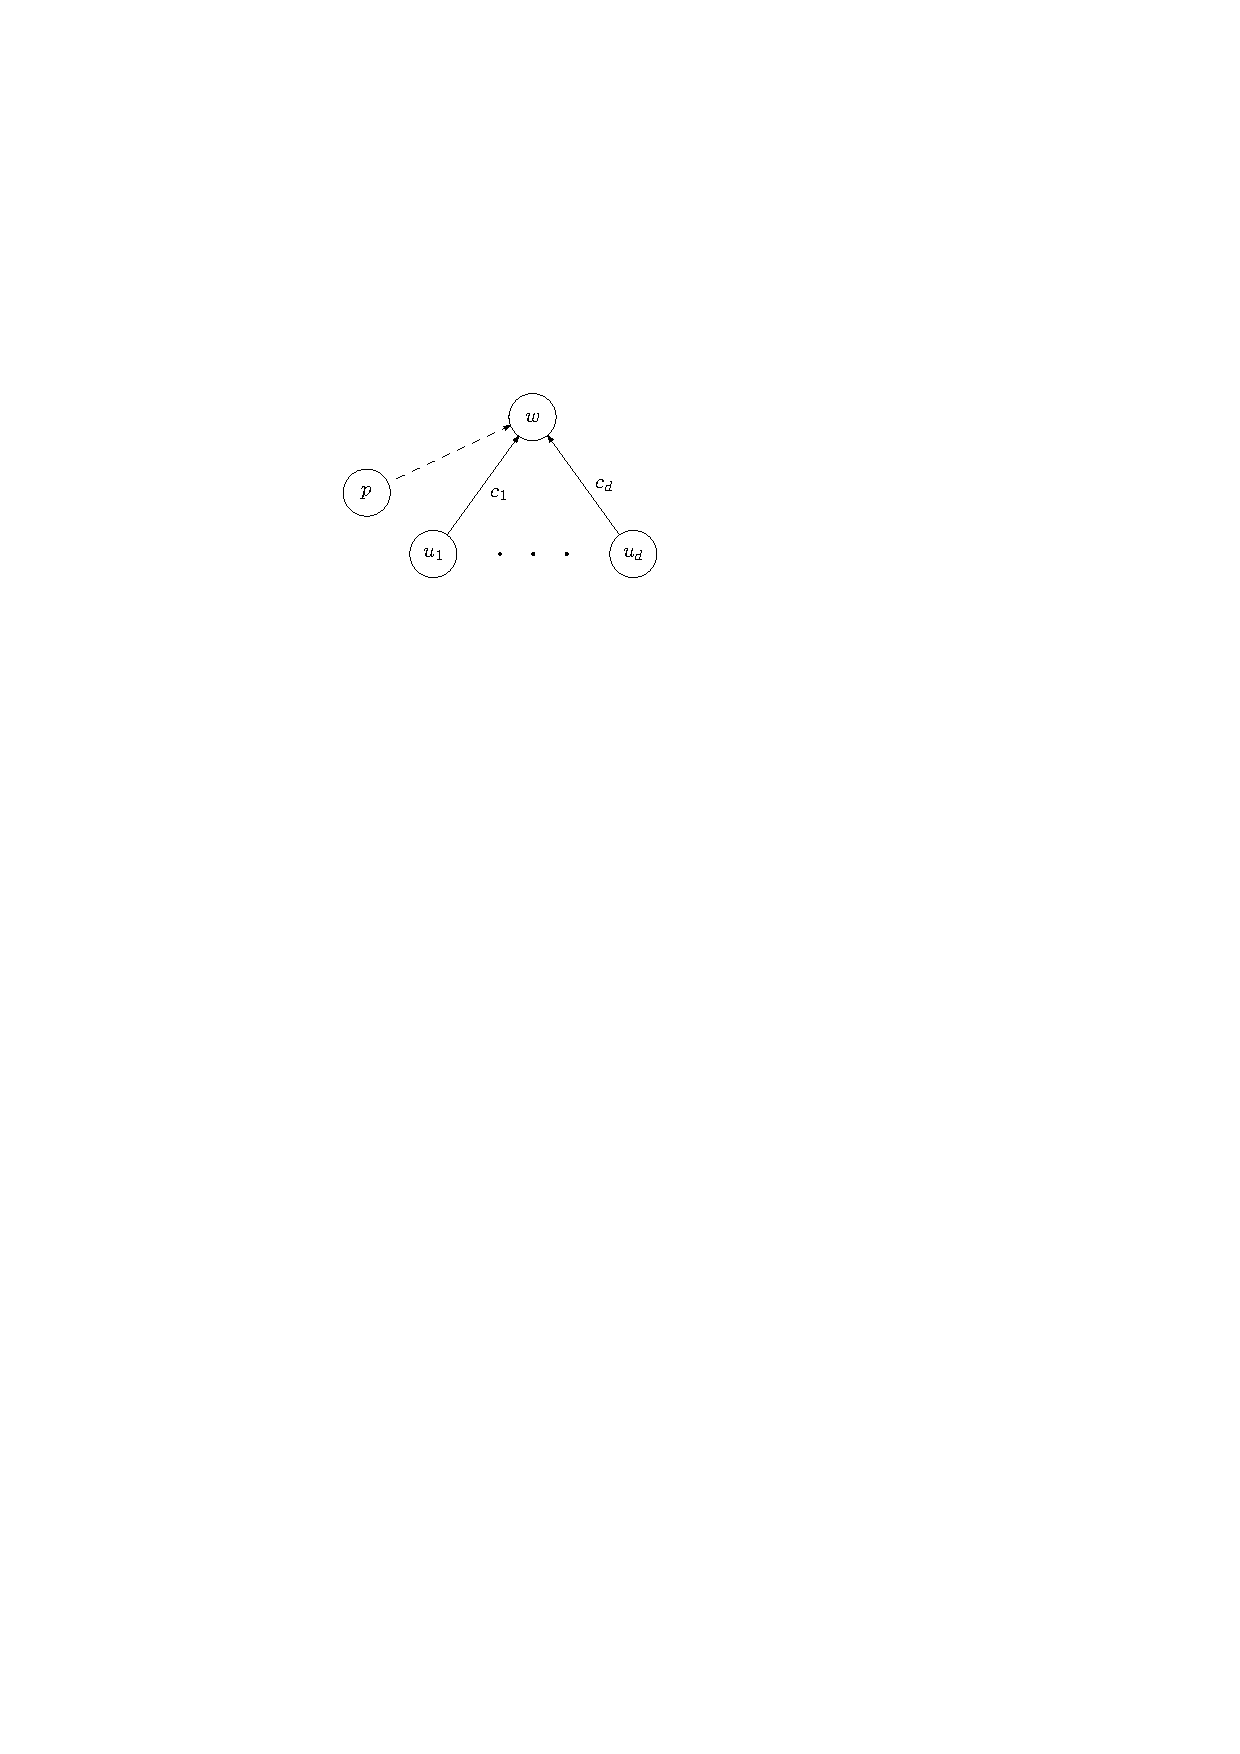
\includegraphics{figures/gsd-qs-triggered}
	\end{center}
	\caption{Illustration of the GSD graph when $\qs$ is triggered at a node $w$. The dashed edge represents a seed dependencey $(p, w)$ and the remaining edges represent encryption queries $c_i \from \operatorname{encrypt}(u_i, w)$.}
	\label{fig:gsd-qs-triggered}
\end{figure}

The proof in \cite{ttkem} simply argued that this is not too likely if these encryptions were made with an IND-CPA secure scheme. In the context of the DHIES scheme we can say more about these encryptions and achieve a better reduction loss.
Let $(\mathbb{G}, q, g) = \mathcal{G}(1^\eta)$.
Let $x_i = \log_g(pk_{u_i})$. Each encryption $c_i$ is a tuple of the form $\langle g^{y_i}, \Pi_s.\enc_{k_i}(s_w) \rangle$ where $y_i \from [q], k_i = \hdh\left(g^{x_i \cdot y_i}\right)$. Now we can again do a case distinction on whether $\hdh$ was queried for (the encoding of) some group element $g^{x_j \cdot y_j}$ or not:
\begin{enumerate}[(i)]
	\item \label{qs-triggered-case-1} If such a query was made, then $\adv$ solved the Diffie-Hellman challenge $(g^{x_j}, g^{y_j})$. (Remember that we assumed that $w$ is the first node for which $\qs$ is triggered and as before if $w$ is safe, then so are the nodes $u_i$. Thus the adversary has not learned the exponent $x_i$ through querying $\hgen(s_{u_i})$ for any $i$.)
	\item \label{qs-triggered-case-2} If no such query was made, then from $\adv$'s perspective all the $k_i$ are independent, uniformly random keys and it still was able to learn $s_w$ from the EAV secure encryptions $\Pi_s.\enc_{k_1}(s_w), \ldots, \Pi_s.\enc_{k_d}(s_w)$.
\end{enumerate}
We can bound the probability of either of these events occurring using hardness of the DDH problem relative to $\mathcal{G}$ and EAV security of $\Pi_s$, respectively.

To this end, we call a group element $h \in \mathbb{G}$ a \emph{hidden Diffie-Hellman key} if $h = pk_u^{y_{u, v}}$, where $(u, v)$ is an edge in the GSD graph, $u$ is safe and $y_{u, v}$ is the exponent chosen in the DHIES encryption of $s_v$ (i.e. $\adv$ was given a ciphertext of the form $\langle g^{y_{u, v}}, \ldots\rangle$ when it queried $\operatorname{encrypt}(u, v)$). Now analogously to above let $\qdh$ the event that $\adv$ queries $\hdh$ on a hidden Diffie-Hellman key, and let $\fdh$ the event that $\adv$ triggers $\qdh$ when $\qs$ has not (yet) been triggered.
\todo{Querying a hidden DH key can also happen when the adversary first queries the group element and then later does an encrypt query that creates an edge with that group element as the key. Add notes in SD-GSD adversaries in proofs to explain how they keep track of this and check if any arguments must be adapted (what is essential is that the adversary has not queried $\hdh(k)$ for any hidden key $k$ and the simulations are thus distributed identically).}
Then we can split the event $\qs$ into two cases as motivated above:
\begin{align*}
	\pr{\qs} & = \pr{\qs \land \fdh} + \pr{\qs \land \overline{\fdh}\,}.
\end{align*}
We bound $\pr{\qs \land \fdh}$ and $\pr{\qs \land \overline{\fdh} \,}$ in Lemma~\ref{lemma:dh-reduction} and Lemma~\ref{lemma:eav-reduction}, respectively. Overall this gives us a bound on the advantage of $\adv$ using \eqref{eq:theorem-sd-gsd-security-win-cases}. (To be precise, the event $\qs \land \fdh$ is a superset of case (\ref{qs-triggered-case-1}) above. However, the argument applied in Lemma~\ref{lemma:dh-reduction} gives the same bound for either event and this more general event has the advantage of being simpler.)

\begin{proof}[of Theorem~\ref{theorem:sdgsd-security}]
	Let $\delta, N$ functions in $\eta$ (mapping to $\N$) with $\delta \le N$.
	Let $\eta$ arbitrary and let $\adv$ an arbitrary SD-GSD adversary constructing a GSD graph of size at most $N(\eta)$ and indegree at most $\delta(\eta)$, making at most $\ms(\eta)$ queries to $\hgen$ or $\hdep$ and at most $\mdh(\eta)$ queries to $\hdh$, each of length at most $\gamma(\eta)$, and running in time $\tilde{t}(\eta)$. We will use the events defined above.

	We first justify step $(\dagger)$ in \eqref{eq:theorem-sd-gsd-security-win-cases}. Note that by the rules imposed on the adversary in the SD-GSD game, the challenge node $v$ is safe and its seed $s_v$ thus indeed hidden. If $\qdep$ does not hold, then $\adv$ has not queried $\hdep$ for $s_v$ and, by virtue of $\hdep$ being a random oracle, $\hdep(s_v)$ is a uniformly distributed value in $\{0, 1\}^\rho$ from $\adv$'s perspective. The value $s$ follows the same distribution. Thus, $\adv$ behaves the same when given either $r = s$ or $r = \hdep(s_v)$ and
	\begin{align} \label{eq:theorem-sd-gsd-security-not-qdep-behavior}
		\begin{split}
			\pr{1 \from \adv \mid \overline{\qdep}, b = 1} & = \pr{1 \from \adv \mid \overline{\qdep}, r = s}          \\
			& = \pr{1 \from \adv \mid \overline{\qdep}, r = \hdep(s_v)} \\
			& = \pr{1 \from \adv \mid \overline{\qdep}, b = 0}.
		\end{split}
	\end{align}
	Therefore
	\begin{align*}
		\pr{\wins \mid \overline{\qdep} \,} & = \begin{aligned}[t]
			                                         & \pr{1 \from \adv \mid \overline{\qdep}, b = 1} \cdot \frac{1}{2}   \\
			                                         & + \pr{0 \from \adv \mid \overline{\qdep}, b = 0} \cdot \frac{1}{2}
		                                        \end{aligned}                                                                             \\
		                                    & \stackrel{\mathclap{\eqref{eq:theorem-sd-gsd-security-not-qdep-behavior}}}{=} \begin{aligned}[t]
			                                                                                                                     & \pr{1 \from \adv \mid \overline{\qdep}, b = 0} \cdot \frac{1}{2}   \\
			                                                                                                                     & + \pr{0 \from \adv \mid \overline{\qdep}, b = 0} \cdot \frac{1}{2}
		                                                                                                                    \end{aligned} \\
		                                    & = \frac{1}{2}.
	\end{align*}

	By Lemma~\vref{lemma:dh-reduction} we have\footnote{Note that we are again omitting the argument $\eta$ from the functions on the right hand side ($N, \eddh$ and $\mdh$ in this case).}
	\[
		\pr{\qs \land \fdh} \le N \cdot \eddh + \frac{\mdh \cdot N^2}{q}.
	\]
	and by Lemma~\vref{lemma:eav-reduction} we have
	\[
		\pr{\qs \land \overline{\fdh}\,} \le \delta \cdot N \cdot \eeav + \frac{\ms \cdot N}{2^\rho},
	\]
	so we know that
	\begin{equation} \label{eq:theorem-sd-gsd-security-qs-bound}
		\pr{\qs} \le N \cdot \eddh + \delta \cdot N \cdot \eeav + \frac{\mdh \cdot N^2}{q} + \frac{\ms \cdot N}{2^\rho} = \tilde{\epsilon}(\eta) / 2.
	\end{equation}
	Then
	\begin{align*}
		\advantage{\Pi}{\eta}{SD-GSD}(\adv) & = 2 \cdot \left(\pr{\wins} - \frac{1}{2}\right)                                                   \\
		                                    & \stackrel{\mathclap{\eqref{eq:theorem-sd-gsd-security-win-cases}}}{\le} \;  2 \cdot \pr{\qs}      \\
		                                    & \stackrel{\mathclap{\eqref{eq:theorem-sd-gsd-security-qs-bound}}}{\le} \; \tilde{\epsilon}(\eta).
	\end{align*}
\end{proof}

\subsubsection{Reducing to EAV security}

Recall case \ref{qs-triggered-case-2} in the high-level discussion of Theorem~\ref{theorem:sdgsd-security}: the adversary $\adv$ was able to learn the seed $s_w$ given the EAV secure encryptions $\Pi_s.\enc_{k_1}(s_w), \ldots, \Pi_s.\enc_{k_d}(s_w)$. We can see $\adv$ as an adversary against a security game where $\adv$ is given $d$ EAV secure encryptions $c_1 \from \Pi_s.\enc_{k_1}(m), \ldots, c_d \from \Pi_s.\enc_{k_d}(m)$ of a message $m$ with $k_i \from \Pi_s.\gen(1^\eta)$ and must compute $m$. If we can prove that beating such a game is hard, then we can bound the probability of $\adv$ actually learning $s_w$ in this way.

This is exactly how we proceed in this section. Instead of asking the adversary to compute an encrypted message $m$, we turn to a more familiar decisional formulation as in the IND-CPA game (where the adversary may choose a pair $m_0, m_1$ and must distinguish whether the $d$ ciphertexts encrypt $m_0$ or $m_1$). We call this security notion \emph{EAV security under multiple (M) independent (I) encryptions of a single (S) pair of messages} (MIS-EAV).

\begin{definition}[The MIS-EAV game]
	Let $\kappa$ denote the security parameter and let $\Pi$ a private-key encryption scheme. Define the game $\game{\Pi}{\kappa}{MIS-EAV}(\adv)$ for an adversary $\adv$:
	\begin{enumerate}[1.]
		\item The adversary $\adv$ outputs $q \in \N$ and a pair of messages $m_0, m_1$ of the same length. We refer to $q$ as the number of \emph{queries} made by $\adv$.
		\item A bit $b \from \{0, 1\}$ is sampled. For each $i \in [q]$, $\adv$ is given an encryption $c_i \from \Pi.\enc_{k_i}(m_b)$ where $k_i \from \Pi.\gen(1^\kappa)$ is generated independently of the other keys.
		\item $\adv$ outputs a bit $b'$. The output of the game is defined to be $1$ if $b' = b$, and $0$ otherwise.
	\end{enumerate}
\end{definition}

\begin{definition}[MIS-EAV security]
	A private-key encryption scheme $\Pi$ is \emph{$(t, \epsilon, q)$-MIS-EAV-secure} if for all $\kappa$, for any adversary $\adv$ making at most $q(\kappa)$ queries and running in time $t(\kappa)$ we have
	\begin{align*}
		\advantage{\Pi}{\kappa}{MIS-EAV}(\adv) \coloneqq 2 \cdot \left(\pr{\game{\Pi}{\kappa}{MIS-EAV}(\adv) = 1} - \frac{1}{2}\right) \le \epsilon(\kappa).
	\end{align*}
\end{definition}

Similar to how IND-CPA security for a single encryption query implies IND-CPA security for $q$ queries with a security loss of $q$ by a standard hybrid argument, one can show that EAV security implies MIS-EAV security with the same loss. To see why, recall the hybrid argument for IND-CPA security (as discussed in e.g. \cite[Theorem 12.6]{introduction-to-modern-cryptography}): We define the sequence of hybrid games $H_0, \ldots, H_q$ where in the game $H_i$ the first $i$ encryption queries encrypt the second message and the remaining $q - i$ queries encrypt the first message. Then given an IND-CPA adversary $\adv$ for multiple encryptions, an IND-CPA adversary $\adv'$ is constructed to bound
\[
	\abs*{\pr{\adv \text{ outputs } 0 \text{ in game } H_{i - 1}} - \pr{\adv \text{ outputs } 0 \text{ in game } H_{i}}}
\]
for arbitrary $i$.
The adversary $\adv'$ simulates $H_{i - 1}$ or $H_{i}$ to $\adv$ depending on whether the ciphertext received from the (single-query) IND-CPA challenger, which gets passed on as the response to the $i$-th query, encrypts the first or the second message from the $i$-th pair of messages. $\adv'$ then uses the encryption oracle to pass on the right encryptions to $\adv$ for all other queries. Now notice that if we wanted to simulate to an MIS-EAV adversary we wouldn't need access to an encryption oracle since for the MIS-EAV security game all the other encryptions can easily be generated by $\adv'$ sampling the new keys itself.

The argument would of course also work without restricting the adversary to a single pair of messages (which we could call MI-EAV security). However, we will make use of this restriction to provide a tighter reduction for a certain class of schemes in the appendix.

\begin{lemma} \label{lemma:mis-eav-from-eav}
	Let $\Pi$ a private-key encryption scheme with finite message space. Let $t_{\gen}, t_{\enc}$ functions in $\kappa$ that upper bound the runtime of $\Pi.\gen$ and $\Pi.\enc$, respectively. If $\Pi$ is $(t, \epsilon)$-EAV-secure, then for any function $q$, $\Pi$ is $(\tilde{t}, q \cdot \epsilon, q)$-MIS-EAV-secure with $\tilde{t} = t - \mathcal{O}(q \cdot (t_\gen + t_\enc))$.
\end{lemma}

The details of the proof can be found in Section~\ref{sec:mis-eav-from-eav-proof} of the appendix.

\begin{lemma} \label{lemma:eav-reduction}
	Recall the assumptions, variables and events from the statement and proof of Theorem~\ref{theorem:sdgsd-security}. In particular, assume that $\Pi_s$ is $(t, \eeav)$-EAV-secure. Let $\eta$ arbitrary and let $\adv$ an SD-GSD adversary constructing a GSD graph of size at most $N(\eta)$ and indegree at most $\delta(\eta)$, making at most $\ms(\eta)$ queries to $\hgen$ or $\hdep$ and at most $\mdh(\eta)$ queries to $\hdh$, and running in time $\tilde{t}(\eta)$. Then
	\[
		\pr{\qs \land \overline{\fdh}\,} \le \delta \cdot N \cdot \eeav + \frac{\ms \cdot N}{2^\rho}.
	\]
\end{lemma}

\paragraph{Intuition} By Lemma~\vref{lemma:mis-eav-from-eav} we know that $\Pi_s$ is MIS-EAV secure. Continuing the high-level argument before the proof of Theorem~\ref{theorem:sdgsd-security}, consider the first moment that $\adv$ triggers $\qs \land \overline{\fdh}$ by querying the seed of some safe node $w$.  As intended, it follows from the definition of the event $\fdh$ that from $\adv$'s perspective all DHIES ciphertexts it got from queries $\operatorname{encrypt}(u, w)$ for any $u$ contain encryptions of $s_w$ under independent, uniformly random keys using $\Pi_s$. Moreover, as already argued once, $\adv$ has learned nothing from a potential seed dependency $(p, w)$, so these encryptions are everything $\adv$ had at its proposal to learn $s_w$.

\todo{Add plot.}

We can use $\adv$'s ability to compute the seed $s_w$ of a safe node $w$ from encryptions of $s_w$ to construct an MIS-EAV adversary: We first guess a node $w$ whose seed $\adv$ may query first. Next we give the MIS-EAV challenger $s_w$ and some other independent seed $s$. We simulate the SD-GSD game to $\adv$ and embed the encryptions from the MIS-EAV challenger when answering queries of the form $\operatorname{encrypt}(u, w)$ for any $u$. Now consider the behavior of $\adv$ depending on which seed the challenger chooses to encrypt:
\begin{itemize}
	\item If the challenger chooses to encrypt $s_w$, then $\adv$ will trigger the event $\qs \land \overline{\fdh}$ with the same probability as before. We can detect whether $\qs \land \overline{\fdh}$ gets triggered since all seeds in the simulation are known. If $\qs \land \overline{\fdh}$ occurs and we guessed $w$ correctly, the event will be triggered at $w$ and $\adv$ will query $s_w$, telling us that the challenger encrypted $s_w$.
	\item If the challenger chooses to encrypt $s$, then $\adv$ receives no information about $s_w$ and has negligible probability of querying it.
\end{itemize}
Thus, the advantage of the MIS-EAV adversary is about $\pr{\qs \land \overline{\fdh}\,}/N$, where the factor $1/N$ arises from guessing $w$, and using that $\Pi_s$ is MIS-EAV secure we can bound this probability. Since we are only interested in checking whether the event was triggered for $w$, the adversary can abort when this is no longer possible ($w$ is corrupted, some other hidden seed is queried, etc.). The details of the proof can be found in Section~\ref{sec:eav-reduction-proof} of the appendix.

For a certain class of schemes, we can improve on Lemma~\ref{lemma:mis-eav-from-eav} and achieve a tight reduction. This allows use to get rid of the factor $\delta$ in Lemma~\ref{lemma:eav-reduction}. However, we do not use this in our main result and refer the interested reader to Section~\ref{sec:tighter-mis-eav-security} of the appendix.

\subsubsection{Reducing to the DDH problem}

\begin{lemma} \label{lemma:dh-reduction}
	Recall the assumptions, variables and events from the statement and proof of Theorem~\ref{theorem:sdgsd-security}. In particular, assume that the DDH problem is $(t, \eddh)$-hard relative to $\mathcal{G}$. Let $\eta$ arbitrary and let $\adv$ an SD-GSD adversary constructing a GSD graph of size at most $N(\eta)$ and indegree at most $\delta(\eta)$, making at most $\ms(\eta)$ queries to $\hgen$ or $\hdep$ and at most $\mdh(\eta)$ queries to $\hdh$, and running in time $\tilde{t}(\eta)$. Then
	\[
		\pr{\qs \land \fdh} \le N \cdot \eddh + \frac{\mdh \cdot N^2}{q}.
	\]
\end{lemma}

\paragraph{Intuition} We will bound the simpler event $\fdh$. This event tells us that there is some safe node $a$ in the GSD graph with encryption edges to nodes $u_1, \ldots, u_d$, where the query $\operatorname{encrypt}(a, u_i)$ returned the ciphertext $\langle g^{y_i}, \Pi_s.\enc_{k_i}(s_{u_i}) \rangle$ with $k_i = \hdh(g^{sk_{a} \cdot y_i})$, such that $g^{sk_a \cdot y_j}$ was the first hidden Diffie-Hellman key queried by $\adv$ for some $j$.
Moreover, at the time $g^{sk_a \cdot y_j}$ was queried, no hidden seed had yet been queried by $\adv$, implying that $\adv$ had not queried $\hgen(s_a)$ and thus had no information about $sk_a$ besides $pk_a$ (recall that $(pk_a, sk_a) = \dhies.\gen(1^\eta, \hgen(s_a))$).

\todo{Add plot.}

It is interesting to note that our approach does not require that $\adv$ has not queried $\hdep$ for a hidden seed (i.e. that $\qdep$ was not triggered) as is implied by the event $\fdh$, because knowing $\hgen(s_a)$ is the only way to learn about $sk_a$. Regardless, we still want to have our definition of $\fdh$ include this information, as the bound on $\pr{\qs \land \overline{\fdh} \,}$ in Lemma~\vref{lemma:eav-reduction} relies on the fact that in the event of $\qs \land \overline{\fdh}$ happening,  $\qdh$ was not yet triggered when the event $\qs$ was triggered, i.e. when either the event $\qgen$ \emph{or} the event $\qdep$ was triggered.

The intuition is clear that this means that $\adv$ solved the Diffie-Hellman challenge $(g^{sk_a}, g^{y_j})$. What is not immediately clear is how to embed a \emph{given} Diffie-Hellman challenge $(g^x, g^y)$  from an instance of the DDH game and use $\adv$ to tell whether the key $k$ chosen by the challenger is the real key $g^{x \cdot y}$ or a uniformly random group element.
An intuitive strategy would be to embed the challenge by setting $pk_a = g^x$ and $g^{y_j} = g^y$, which involves guessing $u_j$, and simply checking whether for any of the queries $q_i$ to $\hdh$ by $\adv$, such that $q_i$ encodes a group element in $\mathbb{G}$, it holds that $q_i = k$. Now:
\begin{itemize}
	\item If $k = g^{x \cdot y}$, $\adv$ triggers $\fdh$ and we guessed $a$ and $u_j$ correctly, then indeed as described above $q_i = g^{sk_a \cdot y_j} = g^{x \cdot y} = k$ will hold for some $i$.
	\item If $k$ is a random group element, then $\adv$ has negligible probability of querying $k$, as no information about $k$ is ever leaked to $\adv$.
\end{itemize}
If we make sure not to change $\adv$'s view of the game in the case $k = g^{x \cdot y}$ in this process, we can achieve an advantage of about $\pr{\fdh} / N^2$, where one factor $1/N$ arises from guessing $a$ and another from guessing $u_j$. Unfortunately, this would yield no improvement over the result from \cite{ttkem}.

To avoid this issue, we can use random self-reducability of the DDH problem and avoid guessing $u_j$. Instead of embedding $g^y$ into a single encryption edge, we embed it into all $d$ encryption edges. To get a uniformly random exponent from $y$ we set $y_j = y + r_j \mod q$ with $r_j \from [q]$. Given $g^{x \cdot y_j}$, we can easily compute $g^{x \cdot y}$:
\[
	g^{x \cdot y_j} = g^{x \cdot (y + r_j)} = g^{x \cdot y}	\cdot g^{x \cdot r_j} \iff g^{x \cdot y} = g^{x \cdot y_j} \cdot \underbrace{((g^x)^{r_j})^{-1}}_{\eqqcolon \, R_j}.
\]
Now to determine whether $k$ is the real Diffie-Hellman key, we check whether $q_i \cdot R_j = k$ for some $i, j$. This yields an advantage of about $\pr{\fdh} / N$ (and a slightly larger runtime). The details of the proof can be found in Section~\ref{sec:dh-reduction-proof} of the appendix.


\section{Our concrete result for TreeKEM}

The following theorem describing the security of TreeKEM, stated informally here, is our main practical result. It bounds the advantage of any adversary creating $c$ commits and $p$ add or update proposals in a group with at most $u$ users in distinguishing the group key of any uncompromised commit from a random bit string.

\begin{theorem}[Informal] \label{theorem:treekem-security-informal}
	If the DHIES scheme is used in TreeKEM, the private-key encryption scheme in DHIES is $(t, \eeav)$-EAV-secure and the DDH problem is $(t, \eddh)$-hard in the Diffie-Hellman group, then for all $c, p, u$, TreeKEM is $(\tilde{t}, \tilde{\epsilon}, c, p, u)$-secure in the ROM with $\tilde{t} \approx t$ and
	\begin{align*}
		\begin{split}
			\tilde{\epsilon} ={} & 2 \cdot u \cdot (3 \cdot c \cdot \log(u) + p) \cdot \eeav \\
			& + 2 \cdot (3 \cdot c \cdot \log(u) + p) \cdot \eddh \\
			& + \mathrm{negl}
		\end{split}
	\end{align*}
	where
	\begin{itemize}
		\item $c$ is the number of commits created
		\item $p$ is the number of add or update proposals created
		\item $u$ is the maximum number of users
		\item the term $\mathrm{negl} = \mathrm{negl}(\eta)$ is negligible and much smaller than the other terms
	\end{itemize}
\end{theorem}

In \cite[Section~\ref*{sec:treekem-security}]{full-version} we restate the above theorem formally as Theorem~\ref*{theorem:treekem-security}. To this end, we also provide formal definitions for the syntax and security of propose and commit CGKA schemes and a high-level description of how to instantiate (the essence of) the TreeKEM protocol with our definitions.

\subsubsection{Security against multiple challenges} As noted in the introduction, although our security definitions only allow the adversary to make a single challenge query, it is straightforward to adapt our proof to show the same security loss with multiple challenge queries. See the note after \cite[Theorem~\ref*{theorem:treekem-security}]{full-version} for details.

\subsection{Interpreting the result}

In the following, we will go through some concrete examples to see what level of security our proof guarantees for TreeKEM with different parameter choices. We will look at the \texttt{MLS\_128\_DHKEMX25519\_AES128GCM\_SHA256\_Ed25519} cipher suite \cite[Section~17.1]{rfc9420} for 128-bit parameters, which uses Curve25519 as the Diffie-Hellman group and AES with a 128-bit key size for private-key encryption. We will assume that both Curve25519 and AES have a 128-bit security level and we will set $(t, \eeav) = (t, \eddh) = (2^{48}, 2^{-80})$.

For 256-bit parameters, we will look at the \texttt{MLS\_256\_DHKEMP521\_AES256GCM\_SHA512\_P521} cipher suite, which uses curve P-521 and 256-bit AES. We will assume that P-521 and 256-bit AES have a 256-bit security level and set $(t, \eeav) = (t, \eddh) = (2^{128}, 2^{-128})$.

\subsubsection{Large groups with hourly commits and frequent updates}

In this example we consider a large group of about 10'000 users, existing for 5 years and making one commit every hour. Then $u \le 2^{14}$ and $c \le 2^{16}$. We also assume that a significant fraction of the users will want to update with every commit. Then, assuming that add proposals are relatively rare, we can bound $p \le c \cdot u = 2^{30}$. This implies $3 \cdot c \cdot \log(u) + p \le 2^{31}$, dominated by $p$.

Then with 128-bit parameters we get
\[
	\et \le 2^{46} \cdot \eeav + 2^{32} \cdot \eddh + \mathrm{negl} \le \frac{1}{2^{33}}
\]
with the $\eeav$ term dominating the result. This only gives a security level of $\tilde{t}/\et \ge 2^{81}$. Since private-key encryption is relatively cheap, using 256-bit AES would have a small impact on the performance and would increase the security level to 95 bits (with the $\eddh$ term now dominating).\footnote{For this we set $(t, \eeav) = (2^{48}, 2^{-208})$.} Finally, using full 256-bit parameters yields 209 bits of security for TreeKEM.

The previous best result in \cite[Theorem 3]{ttkem} proved the bound
\[
	\et \le 2 \cdot (3 \cdot c \cdot \log(u) + p)^2 \cdot \epsilon + \mathrm{negl}
\]
where $\epsilon$ is the IND-CPA security of the underlying public-key encryption scheme. If we assume that DHIES has an $x$-bit security level as a public-key encryption scheme with $x$-bit parameters, the result implies 64 bits of security with 128-bit parameters (with no change when using 256-bit AES) and 192 bits with 256-bit parameters.

\subsubsection{Few updates}

In this example we use the same number of users and commits, but assume that the number of proposals is small such that $p \le c \cdot \log(u)$. In this case, we have $3 \cdot c \cdot \log(u) + p \le 2^{22}$. Then our result guarantees 90 bits of security with 128-bit parameters, 104 bits with 256-bit AES and 218 bits with 256-bit parameters.

In contrast, the bound in \cite{ttkem} implies 82 bits with 128-bit parameters and 210 bits with 256-bit parameters.

\subsubsection{Very large groups with one commit every minute and frequent updates} In this example we consider more extreme values for $c$ and $u$ to highlight the gap between our result and the one in \cite{ttkem}. We assume a group of about 1 million users, existing for 50 years and making one commit every minute. Furthermore, we will again use $p \le c \cdot u$. This means that $u \le 2^{20}$, $c \le 2^{25}$ and $3 \cdot c \cdot \log(u) + p \le 2^{46}$.

These values imply 60 bits of security with 128-bit parameters, 80 bits with 256-bit AES and 188 bits with 256-bit parameters using our result. The result in \cite{ttkem} implies 34 bits of security with 128-bit parameters and 162 bits with 256-bit parameters.


\bibliographystyle{splncs04}
\bibliography{refs}

\appendix

\section{Basic cryptographic definitions} \label{sec:preliminaries-appendix}

\subsection{Encryption schemes}

\subsubsection{Private-key encryption}

\begin{definition}[Private-key encryption {\cite[Definition 3.7]{introduction-to-modern-cryptography}}]
	Let $\kappa$ denote the security parameter. A \emph{private-key encryption scheme} $\Pi$ consists of three probabilistic polynomial-time algorithms $(\gen, \enc, \dec)$ such that:
	\begin{enumerate}[1.]
		\item The \emph{key-generation algorithm} $\gen$ takes as input $1^\kappa$ (in unary) and outputs a key $k$. We will write $k \from \gen(1^\kappa)$.
		\item The \emph{encryption algorithm} $\enc$ takes as input a key $k$ and a message $m \in \{0, 1\}^*$, or $m \in \{0, 1\}^{\le l(\kappa)}$ for some function $l$ if the message space is finite, and outputs a ciphertext $c$. We write this as $c \from \enc_k(m)$.
		\item The deterministic \emph{decryption algorithm} $\dec$ takes as input a key $k$ and a ciphertext $c$, and outputs a message $m$ or $\bot$ (denoting an error). We write this as $m = \dec_{k}(c)$.
	\end{enumerate}

	It is required that for every $\kappa$, every key $k$ output by $\gen$, and every message $m$, it holds that $\pr{\dec_k(\enc_k(m)) = m} = 1$ (where the probability is over the randomness of $\enc_k$).
\end{definition}

\subsubsection{Public-key encryption}

In the following definition we will be more explicit about the randomness used by the algorithm $\gen$, as we will require a way to provide the randomness as input.

\begin{definition}[Public-key encryption {\cite[Definition 12.1]{introduction-to-modern-cryptography}}] \label{def:public-key-encryption}
	Let $\eta$ denote the security parameter.
	A \emph{public-key encryption scheme} $\Pi$ consists of three probabilistic polynomial-time algorithms $(\gen, \enc, \dec)$ such that:
	\begin{enumerate}[1.]
		\item The \emph{key-generation algorithm} $\gen$ takes as input $1^\eta$ (in unary) and outputs a pair of keys $(pk, sk)$ (a public and private key). We will write $(pk, sk) \from \gen(1^\eta)$.

		      The public key defines a message space $\mathcal{M}_{pk}$.

		      The algorithm samples $\rho(\eta)$ uniformly random bits to make randomized decisions for some function $\rho$ polynomial in $\eta$. The sequence of random bits $r \in \{0, 1\}^{\rho(\eta)}$ to be used by the algorithm may also be provided as input. We write this as $(pk, sk) = \gen(1^\eta, r)$ to emphasize the fact that the output is deterministic. The distribution over key pairs output by sampling $r \from \{0, 1\}^{\rho(\eta)}$ and running $\gen(1^\eta, r)$ is identical to the distribution over key pairs output by running $\gen(1^\eta)$.


		\item The \emph{encryption algorithm} $\enc$ takes as input a public key $pk$ and a message $m \in \mathcal{M}_{pk}$, and outputs a ciphertext $c$. We write this as $c \from \enc_{pk}(m)$.
		\item The deterministic \emph{decryption algorithm} $\dec$ takes as input a private key $sk$ and a ciphertext $c$, and outputs a message $m$ or $\bot$ (denoting an error). We write this as $m = \dec_{sk}(c)$.
	\end{enumerate}

	It is required that for every $\eta$, every key $(pk, sk)$ output by $\gen$, and every message $m$, it holds that $\pr{\dec_{sk}(\enc_{pk}(m)) = m} = 1$ (where the probability is over the randomness of $\enc_{pk}$).
\end{definition}

\subsection{Security definitions}

\begin{definition}[The IND-CPA game]
	Let $\kappa$ denote the security parameter and let $\Pi$ a private-key encryption scheme. Define the game $\game{\Pi}{\kappa}{IND-CPA}(\adv)$ for an adversary $\adv$:
	\begin{enumerate}[1.]
		\item A key $k \from \gen(1^\kappa)$ is generated.
		\item The adversary $\adv$ is given oracle access to $\Pi.\enc_k$, and outputs a pair of messages $m_0, m_1$ of the same length.
		\item A bit $b \from \{0, 1\}$ is sampled and $\adv$ is given a ciphertext $c \from \enc_k(m_b)$. ($\adv$ continues to have oracle access to $\Pi.\enc_k$.)
		\item $\adv$ outputs a bit $b'$. The output of the game is defined to be $1$ if $b' = b$, and $0$ otherwise.
	\end{enumerate}
\end{definition}

\begin{definition}[IND-CPA security {\cite[Definition 3.21]{introduction-to-modern-cryptography}}]
	For functions $t, \epsilon$ in the security parameter $\kappa$, a private-key encryption scheme $\Pi$ is \emph{$(t, \epsilon)$-IND-CPA-secure} if for all $\kappa$, for any adversary $\adv$ running in time $t(\kappa)$ we have
	\begin{align*}
		\advantage{\Pi}{\kappa}{IND-CPA}(\adv) \coloneqq 2 \cdot \left(\pr{\game{\Pi}{\kappa}{IND-CPA}(\adv) = 1} - \frac{1}{2}\right) \le \epsilon(\kappa).
	\end{align*}
\end{definition}

We will make use of a weaker form of security called ``indistinguishability in the presence of an eavesdropper'' \cite{introduction-to-modern-cryptography} and will refer to it as ``EAV security''. It is identical to IND-CPA security with the sole exception that the adversary does not have access to an encryption oracle.

\begin{definition}[The EAV game]
	Let $\kappa$ denote the security parameter and let $\Pi$ a private-key encryption scheme. Define the game $\game{\Pi}{\kappa}{EAV}(\adv)$ for an adversary $\adv$:
	\begin{enumerate}[1.]
		\item A key $k \from \gen(1^\kappa)$ is generated.
		\item The adversary $\adv$ outputs a pair of messages $m_0, m_1$ of the same length.
		\item A bit $b \from \{0, 1\}$ is sampled and $\adv$ is given a ciphertext $c \from \enc_k(m_b)$.
		\item $\adv$ outputs a bit $b'$. The output of the game is defined to be $1$ if $b' = b$, and $0$ otherwise.
	\end{enumerate}
\end{definition}

\begin{definition}[EAV security {\cite[Definition 3.8]{introduction-to-modern-cryptography}}]
	A private-key encryption scheme $\Pi$ is \emph{$(t, \epsilon)$-EAV-secure} if for all $\kappa$, for any adversary $\adv$ running in time $t(\kappa)$ we have
	\begin{align*}
		\advantage{\Pi}{\kappa}{EAV}(\adv) \coloneqq 2 \cdot \left(\pr{\game{\Pi}{\kappa}{EAV}(\adv) = 1} - \frac{1}{2}\right) \le \epsilon(\kappa).
	\end{align*}
\end{definition}


\begin{lemma}
	Let $\Pi$ a private-key encryption scheme. If $\Pi$ is $(t, \epsilon)$-IND-CPA-secure, then $\Pi$ is $(t, \epsilon)$-EAV-secure.
\end{lemma}
\begin{proof}
	This follows immediately from the fact that any EAV adversary is also an IND-CPA adversary.
\end{proof}

When analyzing the advantage of an adversary we may make use of the following well known equality.

\begin{lemma}
	Let $X$ a Bernoulli random variable and $b \from \{0, 1\}$ (where $X$ and $b$ are not necessarily independent). Then for $x \in \{0, 1\}$
	\[
		2 \cdot \left(\pr{X = b} - \frac{1}{2}\right) = \pr{X = x \mid b = x} - \pr{X = x \mid b = 1 - x}.
	\]
	In particular, if $\adv$ is an adversary with output in $\{0, 1\}$ playing a game where a bit $b \from \{0, 1\}$ is sampled, then for $x \in \{0, 1\}$
	\begin{equation} \label{eq:advantage-equality}
		2 \cdot \left(\pr{b \from \adv} - \frac{1}{2}\right) = \pr{x \from \adv \mid b = x} - \pr{x \from \adv \mid b = 1 - x}.
	\end{equation}
\end{lemma}
\begin{proof}
	Let $x \in \{0, 1\}$. We have
	\begin{align*}
		2 \cdot \left(\pr{X = b} - \frac{1}{2}\right) & = 2 \cdot \left(\pr{X = x \mid b = x} \cdot \frac{1}{2} + \pr{X = 1 - x \mid b = 1 - x} \cdot \frac{1}{2} - \frac{1}{2}\right) \\
		                                              & = \pr{X = x \mid b = x} + \pr{X = 1 - x \mid b = 1 - x} - 1                                                                    \\
		                                              & = \pr{X = x \mid b = x} - (1 - \pr{X = 1 - x \mid b = 1 - x})                                                                  \\
		                                              & = \pr{X = x \mid b = x} - \pr{X = x \mid b = 1 - x}.
	\end{align*}
\end{proof}

\subsection{The Decisional Diffie-Hellman problem}

\begin{definition}[Group-generation algorithm {\cite[Section 9.3.2]{introduction-to-modern-cryptography}}]
	A \emph{group-generation algorithm} $\mathcal{G}$ is a probabilistic polynomial-time algorithm that takes as input $1^\eta$ and outputs $(\mathbb{G}, q, g)$, where $\mathbb{G}$ is (a description of) a cyclic group with order $q$ and $g \in \mathbb{G}$ is a generator. A group element is represented as a bit-string of length at most $\gamma(\eta)$. We write $(\mathbb{G}, q, g) \from \mathcal{G}(1^\eta)$.
\end{definition}

\begin{definition}[The Decisional Diffie-Hellman (DDH) problem {\cite[Section 9.3.2]{introduction-to-modern-cryptography}}]
	Let $\mathcal{G}$ a group-generation algorithm.
	Define the game $\game{\mathcal{G}}{\eta}{DDH}(\adv)$ for an adversary $\adv$:
	\begin{enumerate}[1.]
		\item $\mathcal{G}(1^\eta)$ is run to obtain $(\mathbb{G}, q, g)$, and exponents $x, y \from [q]$ and a bit $b \from \{0, 1\}$ are sampled.
		\item The adversary $\adv$ is given $\mathbb{G}$, $q$, $g$, $h_1 \coloneqq g^x, h_2 \coloneqq g^y$ and
		      \[
			      k = \begin{cases}
				      g^{x \cdot y} & b = 0 \\
				      \tilde{k}     & b = 1
			      \end{cases}
		      \]
		      where $\tilde{k} \from \mathbb{G}$.
		\item $\adv$ outputs a bit $b'$. The output of the game is defined to be $1$ if $b' = b$, and $0$ otherwise.
	\end{enumerate}
\end{definition}

\begin{definition}[Hardness of the DDH problem {\cite[Definition 9.64]{introduction-to-modern-cryptography}}]
	The DDH problem is \emph{$(t, \epsilon)$-hard relative to} $\mathcal{G}$ if for all $\eta$, for any adversary $\adv$ running in time $t(\eta)$ we have
	\begin{align*}
		\advantage{\mathcal{G}}{\eta}{DDH}(\adv) \coloneqq 2 \cdot \left(\pr{\game{\mathcal{G}}{\eta}{DDH}(\adv) = 1} - \frac{1}{2}\right) \le \epsilon(\eta).
	\end{align*}
\end{definition}

\subsection{The Random Oracle Model} \label{sec:rom}

We will work in the commonly used Random Oracle Model (ROM) to prove our results. We refer the reader to \cite[Chapter 6.5]{introduction-to-modern-cryptography} for an informal overview of the ROM and to \cite{rom} for the original work that introduced the model. The ROM introduces the concept of a \emph{random oracle}. If a function $H : A \to B$ is modelled as a random oracle, then certain assumptions are made about what an adversary $\adv$ knows about $H$ and how it interacts with it:
\begin{itemize}
	\item From $\adv$'s perspective, $H$ is a black-box function. The only way for $\adv$ to interact with $H$ is for it to provide a value $a \in A$ and get back $H(a)$, and this is the only way for $\adv$ to learn $H(a)$. We say that $\adv$ \emph{queries} $H(a)$ or that $\adv$ \emph{queries $H$ for $a$}. This well-defined interface of $\adv$ to $H$ implies that a reduction can extract the queries that $\adv$ makes to $H$.
	\item From $\adv$'s perspective, $H$ is a random variable, sampled u.a.r.\ from the set of all functions from $A$ to $B$. Thus, if $\adv$ queries $H$ for some $a \in A$ that it has not queried before, the value $H(a)$ is a random variable uniformly distributed in $B$ from $\adv$'s perspective.
\end{itemize}
We do not rely on the property known as ``programmability'' in this work.


\section{Appendix}

\subsection{Proof of Lemma~\ref{lemma:mis-eav-from-eav}} \label{sec:mis-eav-from-eav-proof}

\begin{proof}[of Lemma~\ref{lemma:mis-eav-from-eav}] Note that since the message space is finite, the time to encrypt a message is bounded. As outlined before Lemma~\ref{lemma:mis-eav-from-eav}, the lemma follows from a simple hybrid argument. Let $q$ a function in $\kappa$, let $\kappa$ arbitrary and let $\adv$ an arbitrary MIS-EAV adversary running in time $\tilde{t}(\kappa)$ and making at most $q(\kappa)$ queries. Define the sequence of hybrid games $H_0, \ldots, H_q$ where in the game $H_i$ the first $i$ encryptions given to the adversary encrypt $m_1$ and all remaining encryptions encrypt $m_0$. We will write
	\[
		\pr{0 \from \adv \mid H_i}
	\]
	for the probability of $\adv$ outputting $0$ when playing the hybrid game $H_i$.

	Let $i \in [q]$. Construct an EAV adversary $\adv'$ that behaves as follows:
	\begin{enumerate}[1.]
		\item $\adv'$ runs $\adv$ and gets $q, m_0, m_1$.
		\item $\adv'$ outputs the messages $m_0, m_1$ and gets a ciphertext $c$ from the challenger.
		\item $\adv'$ gives the ciphertexts $c_1, \ldots, c_q$ to $\adv$ where
		      \[
			      c_j = \begin{cases}
				      \Pi.\enc_{k_j}(m_1) & i < j \\
				      c                   & i = j \\
				      \Pi.\enc_{k_j}(m_0) & i > j
			      \end{cases}
		      \]
		      and $k_j \from \Pi.\gen(1^\kappa) \; \forall j$.
		\item $\adv'$ outputs whatever bit $\adv$ outputs.
	\end{enumerate}
	Now consider the value of the bit $b$ sampled in $\game{\Pi}{\kappa}{EAV}(\adv')$. If $b = 0$, then the first $i - 1$ ciphertexts that $\adv$ received were encryptions of $m_1$ and the remaining ciphertexts were encryptions of $m_0$, where all encryptions were under keys sampled independently with $\Pi.\gen$. Thus, from the view of $\adv$ everything followed the same distribution as in the game $H_{i - 1}$ and
	\[
		\pr{0 \from \adv' \mid b = 0} = \pr{0 \from \adv \mid H_{i - 1}}.
	\]
	Analogously, in the case $b = 1$ the first $i$ ciphertexts received by $\adv$ were encryptions of $m_1$ and the rest encryptions of $m_0$, so
	\[
		\pr{0 \from \adv' \mid b = 1} = \pr{0 \from \adv \mid H_{i}}.
	\]
	Then
	\begin{align} \label{eq:eav-to-mis-eav-hybrid-distinguisher}
		\begin{split}
			\begin{split}
				\pr{0 \from \adv \mid H_{i - 1}} - & \pr{0 \from \adv \mid H_{i}} \\
				& = \pr{0 \from \adv' \mid b = 0} - \pr{0 \from \adv' \mid b = 1}
			\end{split} \\
			& \stackrel{\mathclap{\eqref{eq:advantage-equality}}}{=} \advantage{\Pi}{\kappa}{EAV}(\adv')                                         \\
			& \le \epsilon
		\end{split}
	\end{align}
	by $(t, \epsilon)$-EAV security of $\Pi$ since $\adv'$ runs in time $\tilde{t} + \mathcal{O}(q \cdot (t_{\gen} + t_{\enc})) = t$.

	Now let $b$ be the bit sampled in the MIS-EAV game. Notice that
	\[
		\pr{0 \from \adv \mid b = 0} = \pr{0 \from \adv \mid H_0}
	\]
	and
	\[
		\pr{0 \from \adv \mid b = 1} = \pr{0 \from \adv \mid H_q}.
	\]
	Then
	\begin{align*}
		\advantage{\Pi}{\kappa}{MIS-EAV}(\adv) & \stackrel{\mathclap{\eqref{eq:advantage-equality}}}{=} \; \pr{0 \from \adv \mid b = 0} - \pr{0 \from \adv \mid b = 1} \\
		                                       & = \pr{0 \from \adv \mid H_0} - \pr{0 \from \adv \mid H_q}                                                             \\
		                                       & = \sum_{i = 1}^{q} \pr{0 \from \adv \mid H_{i - 1}} - \pr{0 \from \adv \mid H_i}                                      \\
		                                       & \stackrel{\mathclap{\eqref{eq:eav-to-mis-eav-hybrid-distinguisher}}}{\le} q \cdot \epsilon.
	\end{align*}
\end{proof}



% 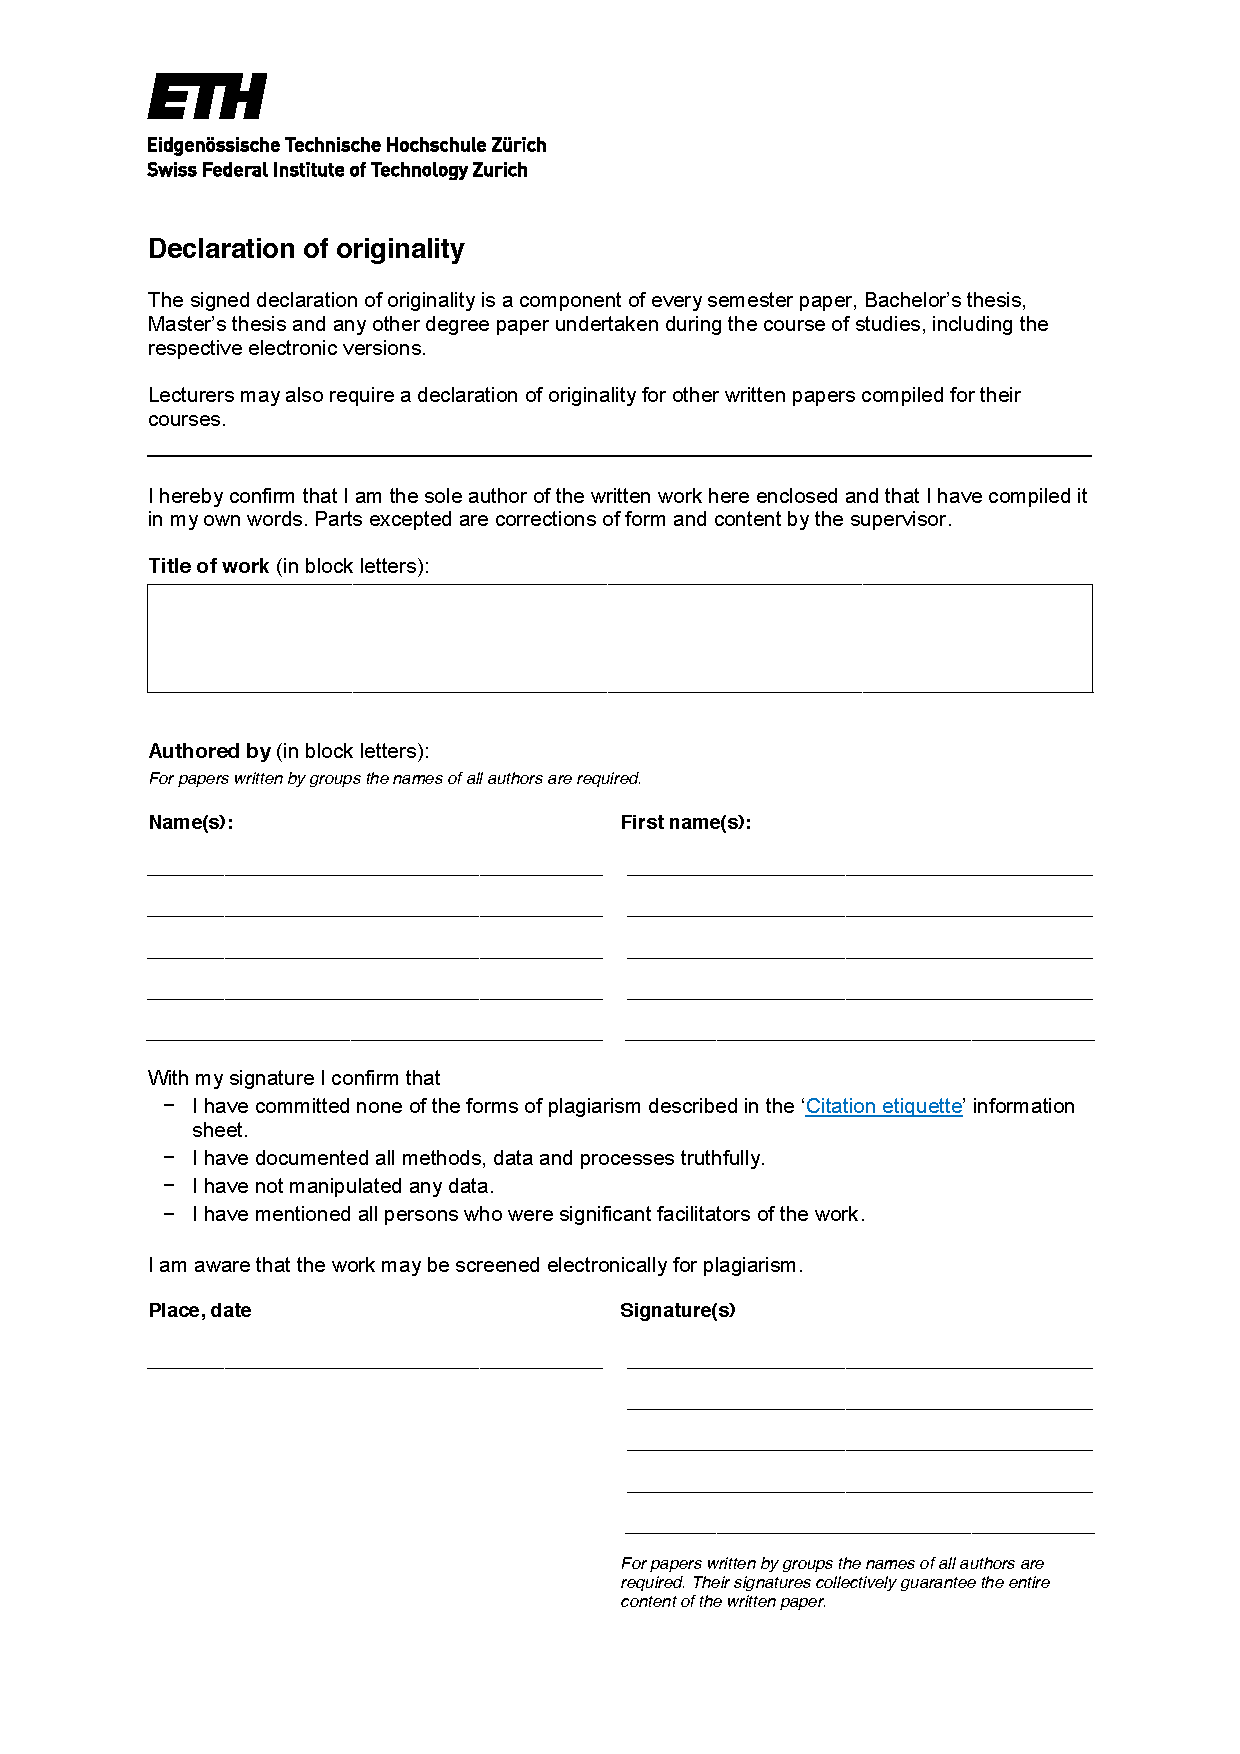
\includepdf[pages={-}]{declaration-originality.pdf}

\end{document}
